\chapter{$B^0$ reconstruction and event selection}

\begin{comment}
\section{Time Dependent \textit{CP} violation measurement}
The measurement of \textit{CP} violation in transitions of 
$B^0$ mesons to their common \textit{CP}
eigenstate $K_S^0 K_S^0 K_S^0$ requires the analysis of the time-dependent differential decay rates. The distribution of events based on the decay time difference $\Delta t$ and flavor is dependent on mixing induced and/or direct \textit{CP} parameters $\mathcal{S}$ and  $\mathcal{A}$. 

\begin{equation}
\mathcal{P}(\Delta t, q ) = 
\frac{e^{-|\Delta t|/\tau_{B^0}}}{4\tau_{B^0}}
\begin{Bmatrix}
1 + q \cdot 
\begin{bmatrix}
\mathcal{S}sin(\Delta M_d \Delta t) + 
\mathcal{A}cos(\Delta M_d \Delta t)
\end{bmatrix}
\end{Bmatrix}
\end{equation}

Here, same as discussed in Chapter 1, $\Delta M_d$ is the mass difference of two $B^0$ mass eigenstates, $\Delta t$ is the decay time difference of signal-side and tag-side $B^0$, namely $\Delta t = t_{CP} - t_{tag}$.  $\tau_B^0$ is the lifetime of $B^0$. And $q = + 1 (-1)$ is the indicator of flavor when tag-side meson is $B^0$ ($\bar{B^0}$). To a good aproximation using Eq(1.47), $\mathcal{A}$ is expected to be zero and $\mathcal{S} = -\text{sin}(2\phi_1)$, given the final states of $K_S^0 K_S^0 K_S^0$ corresponding to \textit{CP}-even ($n_f = + 1$). The previous result from Belle and Babar are shown in Fig 4-1. 

\begin{figure}
\centering 
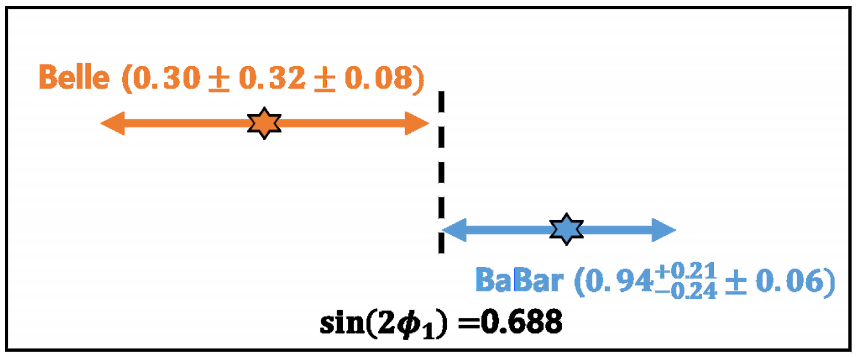
\includegraphics[height=5cm]{belle_babar_result}
\caption{The results of Belle (2007) and Babar on -sin(2$\phi_1$)}
\end{figure}
\end{comment}


%\section{Data Sample and Event Selection}
\begin{comment}
The simulation data (MC) is taken from Belle II official MC campaign 13, named MC13. Both\textit{signal MC} and \textit{signal MC} are produced. In\textit{signal MC}, one of the $B^0$ from $\Upsilon(4S)$ decays into final states 3$K_S^0$ then into 6 charged pions, while the other $B^0$ decays generically using all possible channels. In \textit{signal MC},  $B^0$ from  $\Upsilon(4S)$ all decay generically using all possible channels.
The\textit{signal MC} sample is produced by EvtGen package with provided ``decay.dec" file that describes the required decay mode and branching fraction. As $K_S^0 \to \pi^0 \pi^0$ leads to large background with poor vertex quality, only the final states to 6 charged pions is used.
\end{comment}

As introduced in section 2.9, the branching fraction of $B^0 \to K_S^0  K_S^0  K_S^0)$ is $6.0 \times 10^{-6}$. The simulation sets the $\Upsilon(4S)$ as the mother particle then $\Upsilon(4S)$ decays into to two scalar $B^0$ mesons with mixing. $B^0 \to K_S^0  K_S^0  K_S^0$ decay process is simulated based on the possible phase-space the final state particles could obtain, where no $\it{CP}$ violation is implemented in the generator level, meaning that the input of $\mathcal{S}$(sin2$\phi_1$) and $\mathcal{A}$ are both zero. 
\section{$K_S^0$ Selection}
$K_S^0$ is first reconstructed by the cut-based method using two charged pions which contains a large fraction of fake candidates, as discussed in chapter 3 and Table \ref{tab:kspipi_select}. In addition, a cut on $K_S^0$ is used considering momentum distribution of $B^0 \to K_S^0  K_S^0  K_S^0$, where the huge fake $K_S^0$ appear in low momentum region. Only the $K_S^0$ candidates with momentum larger than 0.05 GeV are selected, as shown in Figure \ref{fig:ks-p}. To further reduce the fake candidates in $K_S^0$ using \textit{KsFinder}, only $K_S^0$ with \textit{FBDT\_Ks} larger than 0.74 are kept.
\begin{figure}[ht]
	\centering
	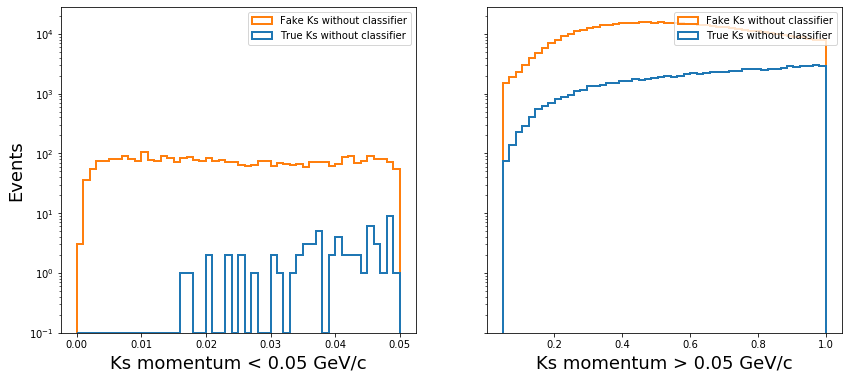
\includegraphics[width=1\linewidth]{ks-p}
	\caption{The distribution of $K_S^0$ momentum. Candidates smaller than 0.05GeV/c are rejected.}
	\label{fig:ks-p}
\end{figure}
%The vertex fit of $K_S^0$ is performed using \textit{TreeFit}. 

\begin{comment}
If we check out the distribution of fitted invariant mass based on SVD hits number associated with daughter tracks as section 3.1 discussed, \textit{SVD00} $K_S^0$ shows a large dispersion from the central region of the distribution of invariant mass after vertex fit, while \textit{SVD11} $K_S^0$ shows a small dispersion as shown in Figure \ref{fig:invm1}. Therefore, considering the $K_S^0$ candidates with different SVD hits, see Figure \ref{fig:ks-r-svdxx} and Table \ref{tab:svdxx}, reflecting the different tracking quality of daughter $\pi^{\pm}$, the different cut on invariant mass M$_{\pi^+\pi^-}$ after vertex fit is applied depending on the SVD hits number of pion tracks. As shown in Figure \ref{fig:invm}, the sideband regions where fake $K_S^0$ is much higher than true $K_S^0$ are excluded. The cut windows are listed in Table \ref{tab:ks_invm}. This improves the reconstruction purity.
\end{comment}
 
 
 


\section{$B^0$  Reconstruction}
By combining three $K_S^0$ particles from selected $K_S^0$ candidates, $B^0$ candidates can be reconstructed. The beam-constraint mass $M_{bc}$ and energy difference $\Delta E$ are used to extract signal, as defined in Equation \ref{eq:mbc} and \ref{eq:dE}, respectively. 

\begin{equation}\label{eq:mbc}
M_{bc} = \sqrt{\frac{s}{4}-p^{*2}_B} 
\end{equation}
\begin{equation}\label{eq:dE}
\Delta E = E^*_B - \frac{\sqrt{s}}{2}
\end{equation}
For $M_{bc}$, $\sqrt{s}$ is defined as the invariant mass of the center-of-mass which is calculated from the beam energies and $p^*_B$ is the reconstructed $B$ momentum in the center-of-mass frame. For $\Delta E$, $E^*_B$ is the reconstructed energy in the center-of-mass frame. These two variables are quite useful for discriminating signal and background events for hadronic $B$ decay with fully reconstructed final states.

 In Belle II, the $B^0$ candidates with $M_{bc} > 5.2$ GeV and $|\Delta{E}| < 0.2$ GeV are required. The vertex information of the fully reconstructed $B^0 \to K_S^0  K_S^0  K_S^0$, called as $\it{CP}$-side, is obtained by the vertex fit using \textit{TreeFit} and the $\chi^2$ probability of the fit is calculated.  Only $B^0$ candidates with converged vertex fit results are kept by a very loose cut of  $P(\chi^2)> 0.001$. On the other hand, the $\it{CP}$ violation measurement does not require the certain decay mode of the other $B^0$ meson in the Rest-Of-Event. The $B$ meson in the Rest-Of-Event is called as tag-side $B$ since this $B$ is used to tag the flavor of $\it{CP}$-side $B$. Thus, no full $B^0$ reconstruction on the tag-side is performed, meaning that the vertex information can not be obtained by the specific final states. Considering this strategy, the vertex fit on the tag-side is done by \textit{KFit} that only takes advantage of well-reconstructed charged particle tracks. The vertex on the tag-side are required to be located inside the standard PXD region, despite that PXD is not fully installed yet. In future, such requirement is subjected to be modified by the PXD hits requirements. 
 
 After performing the vertex fit for both $\it{CP}$-side and tag-side, we check the potential impact of applying \textit{KsFinder} on the reconstructed vertex positions, as well as the impact on the $M_{bc}$ and $\Delta E$. It is necessary for mainly two reasons. First, the \textit{KsFinder} might change the original distributions of $M_{bc}$ and $\Delta E$ of $B^0$ candidates, which are used for the signal extraction. The signal extraction will provide the signal fraction information that is used during the $\it{CP}$ parameters measurement. Second, the \textit{KsFinder} might introduce the bias on the distribution of the vertex positions of $B^0$. The $K_S^0$ candidates with less SVD hits on their daughter pion tracks usually have poorer reconstruction quality and more likely to be rejected as fake candidates. Therefore, we check the distribution of $M_{bc}$ and $\Delta E$ before and after the applying \textit{KsFinder}, as well as the distribution of vertex positions on the $z$-axis. The details about the comparison can be found in the Appendix E. In conclusion, applying \textit{KsFinder} have a negligible impact on $M_{bc}$, $\Delta E$ and the vertex positions on the $z$-axis. The contribution of \textit{KsFinder} as a possible systematic uncertainty source mainly comes from the different data and MC responses of the $K_S^0$ classification, as discussed in the section 3.2.7. 
 
When multiple $B^0$ candidates are obtained in a single event, the best candidates selection (BCS) is performed by ranking their $\chi^2$ of the $\it{CP}$-side vertex fit. Since the BCS is based on the $\chi^2$ that might introduce bias in the vertex positions for $\it{CP}$ fit, we check the distribution of the vertex $\chi^2$, as shown in Figure \ref{fig:b0dist} top left where the data and \textit{generic MC} present a good consistence within $1\sigma$ on average. The distribution of the candidate number per event without BCS is shown in top right of Figure \ref{fig:b0dist} as well, showing an agreement between data and \textit{generic MC} within 1$\sigma$. The distribution of the candidate number per event from the \textit{signal MC} is also in the bottom left of Figure \ref{fig:b0dist}. The 2D distribution of $M_{bc}$ and $\Delta E$ from $B^0 \to K_S^0  K_S^0  K_S^0$ \textit{signal MC} is shown in Figure \ref{fig:b0dist}  bottom right, where the correlation factor is about 15\% between two observables. 
 
\begin{figure}[htpb]
	\begin{minipage}[b]{0.5\linewidth}
		\centering 
		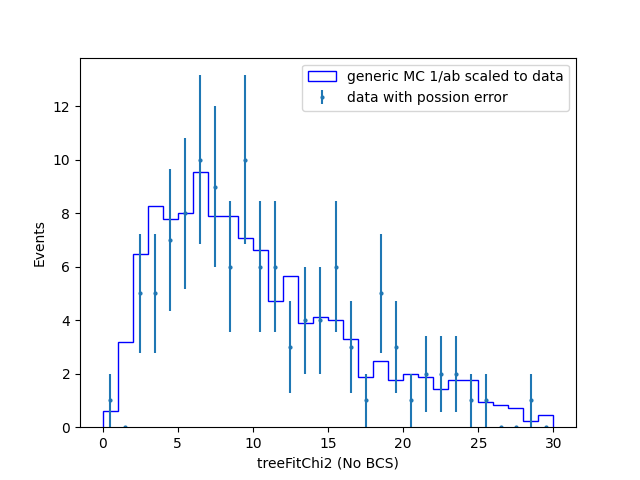
\includegraphics[width=1\linewidth, height=6cm]{figures/best_treeFitChi2_noBCS}
		
	\end{minipage}
	\begin{minipage}[b]{0.5\linewidth}
		\centering 
		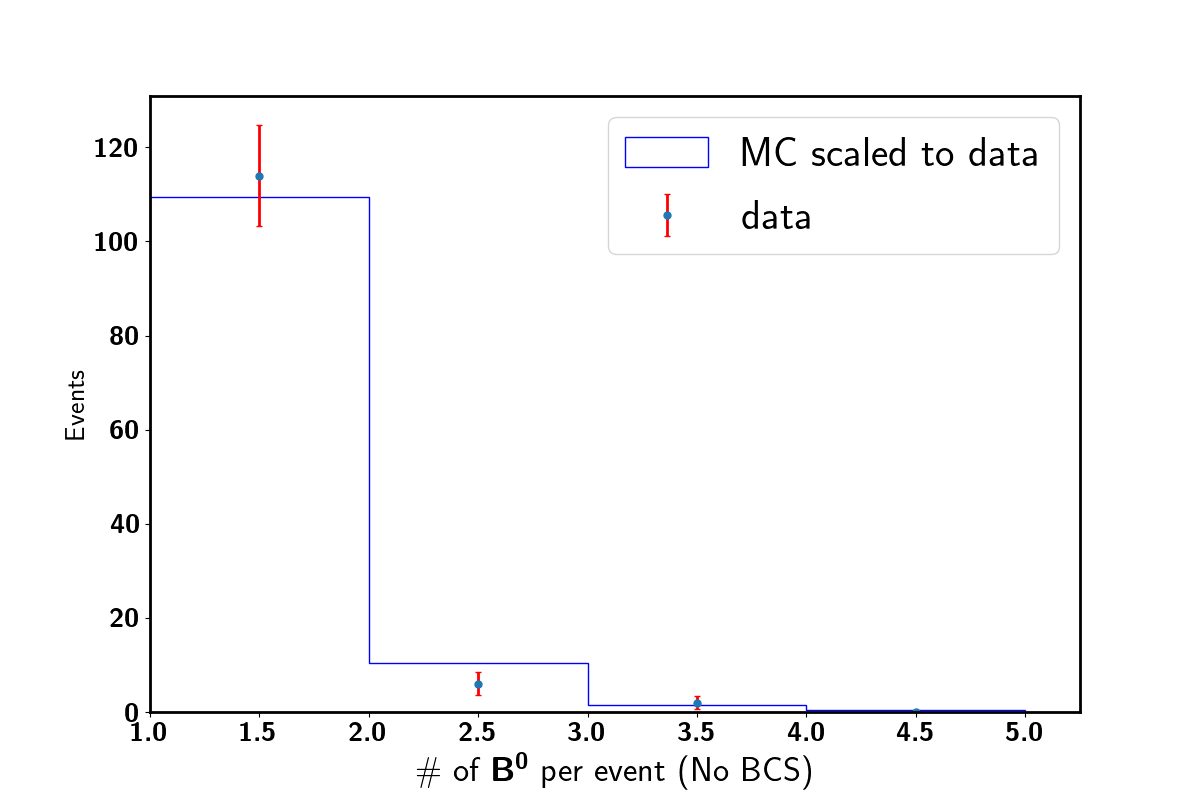
\includegraphics[width=1\linewidth, height=6cm]{figures/best_ncands_noBCS}
		
	\end{minipage}
	\begin{minipage}[b]{0.5\linewidth}
		\centering 
		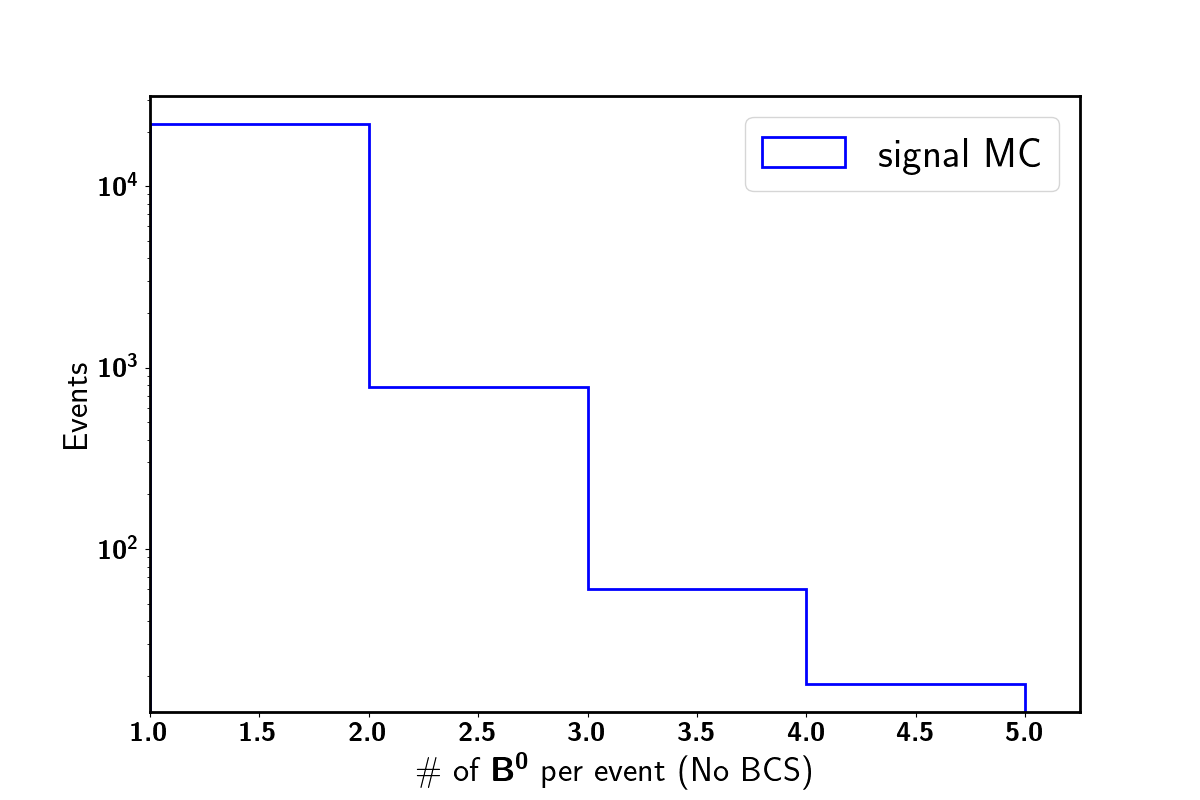
\includegraphics[width=1\linewidth, height=6cm]{figures/best_ncands_sig}
		
	\end{minipage}
	\begin{minipage}[b]{0.5\linewidth}
		\centering 
		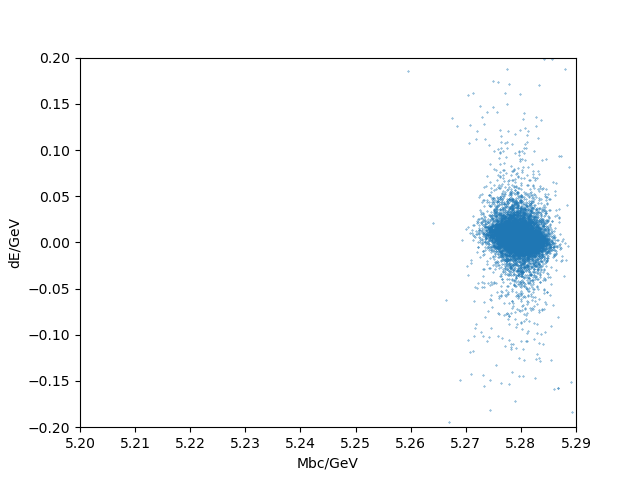
\includegraphics[width=1\linewidth, height=6cm]{figures/hist_sig_MC_Mbc_dE}
		
	\end{minipage}
	
	\caption{Top left is the $\chi^2$ for data and \textit{generic MC} before BCS. Top Right is the $B^0$ candidates per event in data and \textit{generic MC} before the BCS. Bottom left is the number of $B^0$ candidates per event from \textit{signal MC}. Bottom right is the 2D $M_{bc}$ and $\Delta E$ distribution from \textit{signal MC}.}
	\label{fig:b0dist}
\end{figure}
% move to after CS
\section{Continuum Suppression}
The generic decay of $\Upsilon$(4S) produces neutral and charged $B$ mesons, as well as other flavor mesons $q\bar{q}$. Since the branching fraction of $B^0 \to K_S^0  K_S^0  K_S^0$ is relatively low, the $B^0$ candidates after the reconstruction contains a large fraction of fake ones if no special reduction on $q\bar{q}$ is applied. 
The $q\bar{q}$ background events are distributed as a continuum-like shape in the distribution of $M_{bc}$ and $\Delta E$. This calls a demand to distinguish $B\bar{B}$ decay events from $q\bar{q}$ events, which is called as continuum suppression (CS). The rejection is essential because it's the dominated background in this analysis. The most useful information to reject $q\bar{q}$ events is to use the event shape information. In a $B\bar{B}$ event, two mesons are produced almost at rest in the CMS frame since the resonance state $\Upsilon(4S)$ is just slightly lighter than the beam energy. As a result, decay products are emitted more isotropically compared to continuum background events which are more jet-like, back-to-back flying out from the interaction region. The ARGUS and CLEO collaboration~\cite{Bevan_2014} developed a set of variables to suppress the continuum background, which has also been implemented into BASF2 framework. The two major sets of variables are the CLEO cone momentum and the modified Super Fox-wolfram momentum.

CLEO cone momentum can be presented as Equation \ref{eq:ln}, where $ p_i $ is momentum of i-th particle in the Rest-Of-Event. The particles used in a reconstructed $\it{CP}$-side $B^0$ are therefore excluded. The $\theta_i$ is an angle against momentum thrust of reconstructed $\it{CP}$-side \textit{B} meson. The angle is divided into the binned intervals in nine cones of 10 degrees around the thrust.  The $L_n$ stands for the combination that includes particles in a certain cone.  
\begin{equation}\label{eq:ln}
L_n = \sum_{i\in ROE}^{} p_i \times |\text{cos}\theta_i|
\end{equation}

\begin{figure}[htpb]
\centering
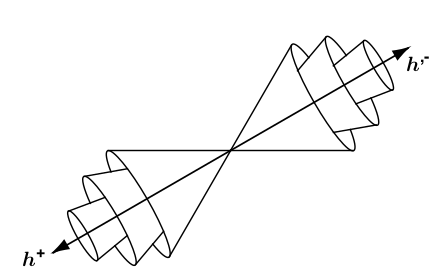
\includegraphics[width=0.8\linewidth]{cleocone}
\caption{A graphical illustration of the CLEO cone. The $h^+$ and $h^{'-}$ present the hadronic tracks from a $B$ decay. The first three cones are drawn~\cite{Bevan_2014}. The nine CLEO cone momentum can be calculated using the particles in each cone. }
\label{fig:cleocone}
\end{figure}
The modified Super Fox-wolfram momentum (KSFW momentum) can be defined as shown in Equation \ref{eq:ksfw}.
\begin{equation}\label{eq:ksfw}
KSFW = \sum_{l=0}^{4}( R_l^{so} + R_l^{oo}) + \gamma \sum_{n=1}^{N_t}|P(t)_n|
\end{equation} 
The $R_l^{so}$ and $R_l^{oo}$ are the functions which depend on both $\it{CP}$ and tag-side particles. Their values are also affected by whether $l$ is even or odd. The $P(t)_n$ is the scalar sum of the transverse momentum of
each particle multiplied by a free parameter $\gamma$ and $N_t$ is
the total number of particles. The detailed  definition for each KSFW momentum is described in Ref~\cite{bevan2017physics}.


\begin{comment}

where the first term is shown in Equation \ref{eq:rlso}.
\begin{equation}\label{eq:rlso}
R_l^{so} = \frac{\alpha_{cl}H_{cl}^{so} +
				\alpha_{nl}H_{nl}^{so}+
			\alpha_{ml}H_{ml}^{so}}{E^*_{beam}-\Delta E}
\end{equation}

when l is odd in Equation \ref{eq:rlso}: 
\begin{equation}
	H_{nl}^{so}=H_{ml}^{so}=0
\end{equation}
and $H_{cl}^{SO}$ is defined as shown in Equation \ref{eq:hclso}: 
\begin{equation}\label{eq:hclso}
	H_{cl}^{so} = \sum_i \sum_{jx}Q_i Q_{jx}|p_{jx}|P_l(cos\theta_{i,jx})
\end{equation}
\textit{i} runs over \textit{B} daughter particles and \textit{jx} for other particles in ROE. \textit{Q} is charge and $p_{jx}$ is momentum for each particle. $P_l(cos\theta_{i,jx})$ is the \textit{i}-th order Legendre polynomial of cosine of \textit{i} and \textit{jx}-th particles.
On the other hand, for \textit{l} is even, $H_{xl}^{SO}$ can be written in Equation \ref{eq:hxlso}.
\begin{equation}\label{eq:hxlso}
	H_{xl}^{so}=\sum_i \sum_{jx}|p_{jx}|P_l(cos\theta_{i,jx})
\end{equation}
The second term in Equation \ref{eq:ksfw}, when \textit{l} is odd, can be defined as Equation \ref{eq:roo}.
\begin{equation}\label{eq:roo}
	R^{oo}_l = \sum_j \sum_k \beta_l Q_j Q_k |p_j||p_k|P_l(cos\theta_j,k)
\end{equation}
\textit{j} and \textit{k} runs over ROE particles and others are same as Equation \ref{eq:hclso}.
For an even \textit{l}: 
\begin{equation}
	R^{oo}_l = \sum_j \sum_k \beta_l |p_j||p_k|P_l(cos\theta_j,k)
\end{equation}
$\beta$ is Fisher coefficients to be determined. 
\end{comment}


\begin{comment}
Besides, two other variables, cos$\theta_B$ and $\Delta Z$, are also quite useful for CS, where the former is the cosine of the angle between $B$ momentum and the beam direction and the latter is the distance between $\it{CP}$ and tag-side $B$ vertices along the beam direction. Both of them are calculated in the CMS frame.
Using these two variables and KSFW momentum, we can form the possibility density functions in the signal and continuum background events. The product of the probability density values for each event is presented as a likelihood of being signal or background, as shown in the Equation \ref{eq:Lsb}. Then we can calculate a ratio $\mathcal{R}$ as Equation \ref{eq:Rcs} shows. It is clear that for a event with very high probability of being a signal, $\mathcal{R}$ is close to 1.

\begin{equation}\label{eq:Lsb}
L_{S/B} = P(KSFW)_{S/B} \times P(cos\theta_B)_{S/B} \times P(\Delta Z)_{S/B}
\end{equation}

\begin{equation}\label{eq:Rcs}
\mathcal{R} = \frac{L_S}{L_S+L_B}
\end{equation}

\end{comment}

In addition to the CLEO cone and KSFW momentum, a few other variables that are related to the event-shape topology are also used in the Belle II CS framework in order to obtain a better continuum background rejection performance. 
This includes $R_2$, $cosTBz$, $cosTBTO$, $thrustOm$, and $thrustBm$.
$R_2$ is defined as the normalized second Fox-Wolfram moment ratio, which is widely used in the decay shape studies.
The $cosTBTO$ is cosine of angle between thrust axis of the $\it{CP}$-side $B$ meson and thrust axis of Rest-Of-Event.
The $cosTBz$ is cosine of angle between thrust axis of the $\it{CP}$-side $B$ meson and $z$-axis.
The $thrustOm$ and $thrustBm$ are the magnitude of the $\it{CP}$-side $B$ thrust axis and Rest-Of-Event thrust axis, respectively. 


 


\begin{figure}[htpb]
	\centering
	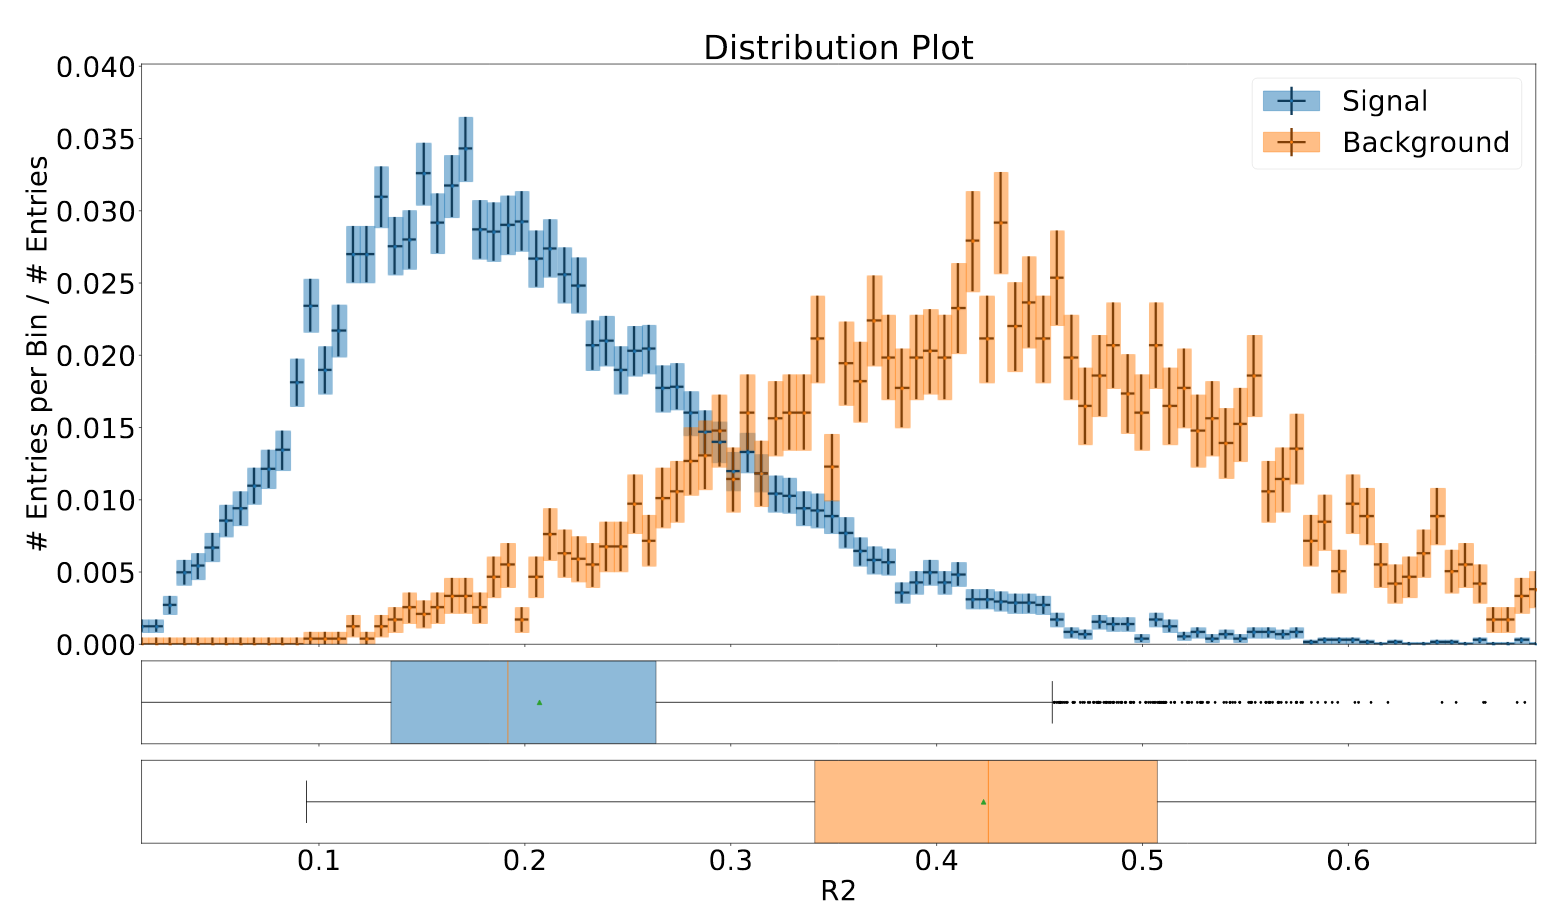
\includegraphics[width=0.7\linewidth]{r2}
	\caption{$R_2$ is the ratio of the second to the zeroth KSFW momentum in Equation \ref{eq:ksfw} of which the distribution in \textit{signal MC} sample which serves as the highest weight as a variable in discriminating the continuum events, having a quite different distribution between signal and background.}
	\label{fig:R2}
\end{figure}

For the Belle II CS strategy, the default method is to use the above variables as an input for a FastBDT classifier to discriminating the signal and continuum background. Such function is implemented by the BASF2. For the specific decay mode $B^0 \to K_S^0  K_S^0  K_S^0$, the training and testing sample prepared from \textit{signal MC} and \textit{generic MC} are used. The target variable of the training is the continuum event truth named $NotContinuumEvent$, where for signal(continuum background) the value is 1(0).  The same events reconstruction procedures for $B^0$ is applied for both MC samples. Events passing the selection using $M_{bc}$ and $\Delta E$ are used for training the CS classifier. The fraction of signal and background is set to 1:1. The output of CS classifier is called \textit{FBDT\_CS}.  We determine the cut value at 0.66 based on the maximum of \textit{FOM} curve, as shown in Figure \ref{fig:cs_fom}. The input variables are listed in Table \ref{tab:cs_abr} with their abbreviations in the training. After the training, the importance of the input variables can be evaluated, shown as Figure \ref{tab:cs_imp-h}.

\begin{figure}[htpb]
	\centering
	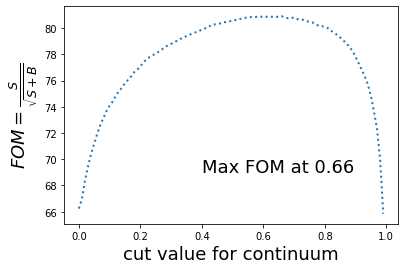
\includegraphics[width=0.6\linewidth]{cs-fom}
	\caption{\textit{FOM} depending on the cut value of continuum classifier output, cut value at 0.66 is used for continuum suppression. }
	\label{fig:cs_fom}
\end{figure}

\begin{figure}[htpb]
	\centering 
	\caption{The importance rank of the input variables for the Belle II CS framework.}
	\label{tab:cs_imp-h}
	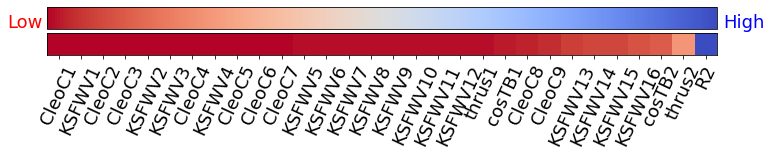
\includegraphics[width=0.9\linewidth]{cs-imp-h}
\end{figure}

The correlation between these training variables are shown in Figure \ref{fig:cs_cor} which are varied between signal and continuum background events. The ROC curve and the efficiency/purity with respect to the classifier output are shown in Figure \ref{fig:cs_roc}, yielding a close performance.
\begin{table}[htpb]
	\begin{minipage}[t]{1\linewidth}
		\centering
		\caption{Input variables and the abbreviations in the continuum suppression framework of BASF2.}
		\label{tab:cs_abr}
		\begin{tabular}{c|c}
			\hline
			Observables &  Abbreviations\\
			\hline
			CleoConeCS(9,) &  CleoC1 \\
			KSFWVariables(hoo1,) & KSFWV1 \\
			CleoConeCS(7,) & CleoC2\\
			CleoConeCS(5,) & CleoC3\\
			KSFWVariables(hso22,) & KSFWV2\\
			KSFWVariables(hoo3,) & KSFWV3\\
			CleoConeCS(4,) & CleoC4 \\
			KSFWVariables(hoo4,) &  KSFWV4\\
			CleoConeCS(3,) & CleoC5 \\
			CleoConeCS(6,) & CleoC6\\
			CleoConeCS(8,) & CleoC7\\
			KSFWVariables(hso14,) &   KSFWV5\\
			KSFWVariables(hso00,) & KSFWV6\\
			KSFWVariables(et,) & KSFWV7\\
			KSFWVariables(hso24,) & KSFWV8\\
			KSFWVariables(hso04,) & KSFWV9\\
			KSFWVariables(hso20,) & KSFWV10 \\
			KSFWVariables(mm2,)  & KSFWV11\\
			KSFWVariables(hoo2,) &  KSFWV12\\
			thrustOm & thrus1 \\
			cosTBz & cosTB1\\
			CleoConeCS(1,) & CleoC8 \\
			CleoConeCS(2,) & CleoC9 \\
			KSFWVariables(hso02,) &  KSFWV13\\
			KSFWVariables(hoo0,) &  KSFWV14 \\
			KSFWVariables(hso12,) &  KSFWV15\\
			KSFWVariables(hso10,) & KSFWV16\\
			cosTBTO & cosTB2\\
			thrustBm & thrus2\\
			R2 & R2\\
			\hline
		\end{tabular}
	\end{minipage}
\end{table}

\begin{figure}[htpb]
	\begin{minipage}[b]{0.5\linewidth}
		\centering 
		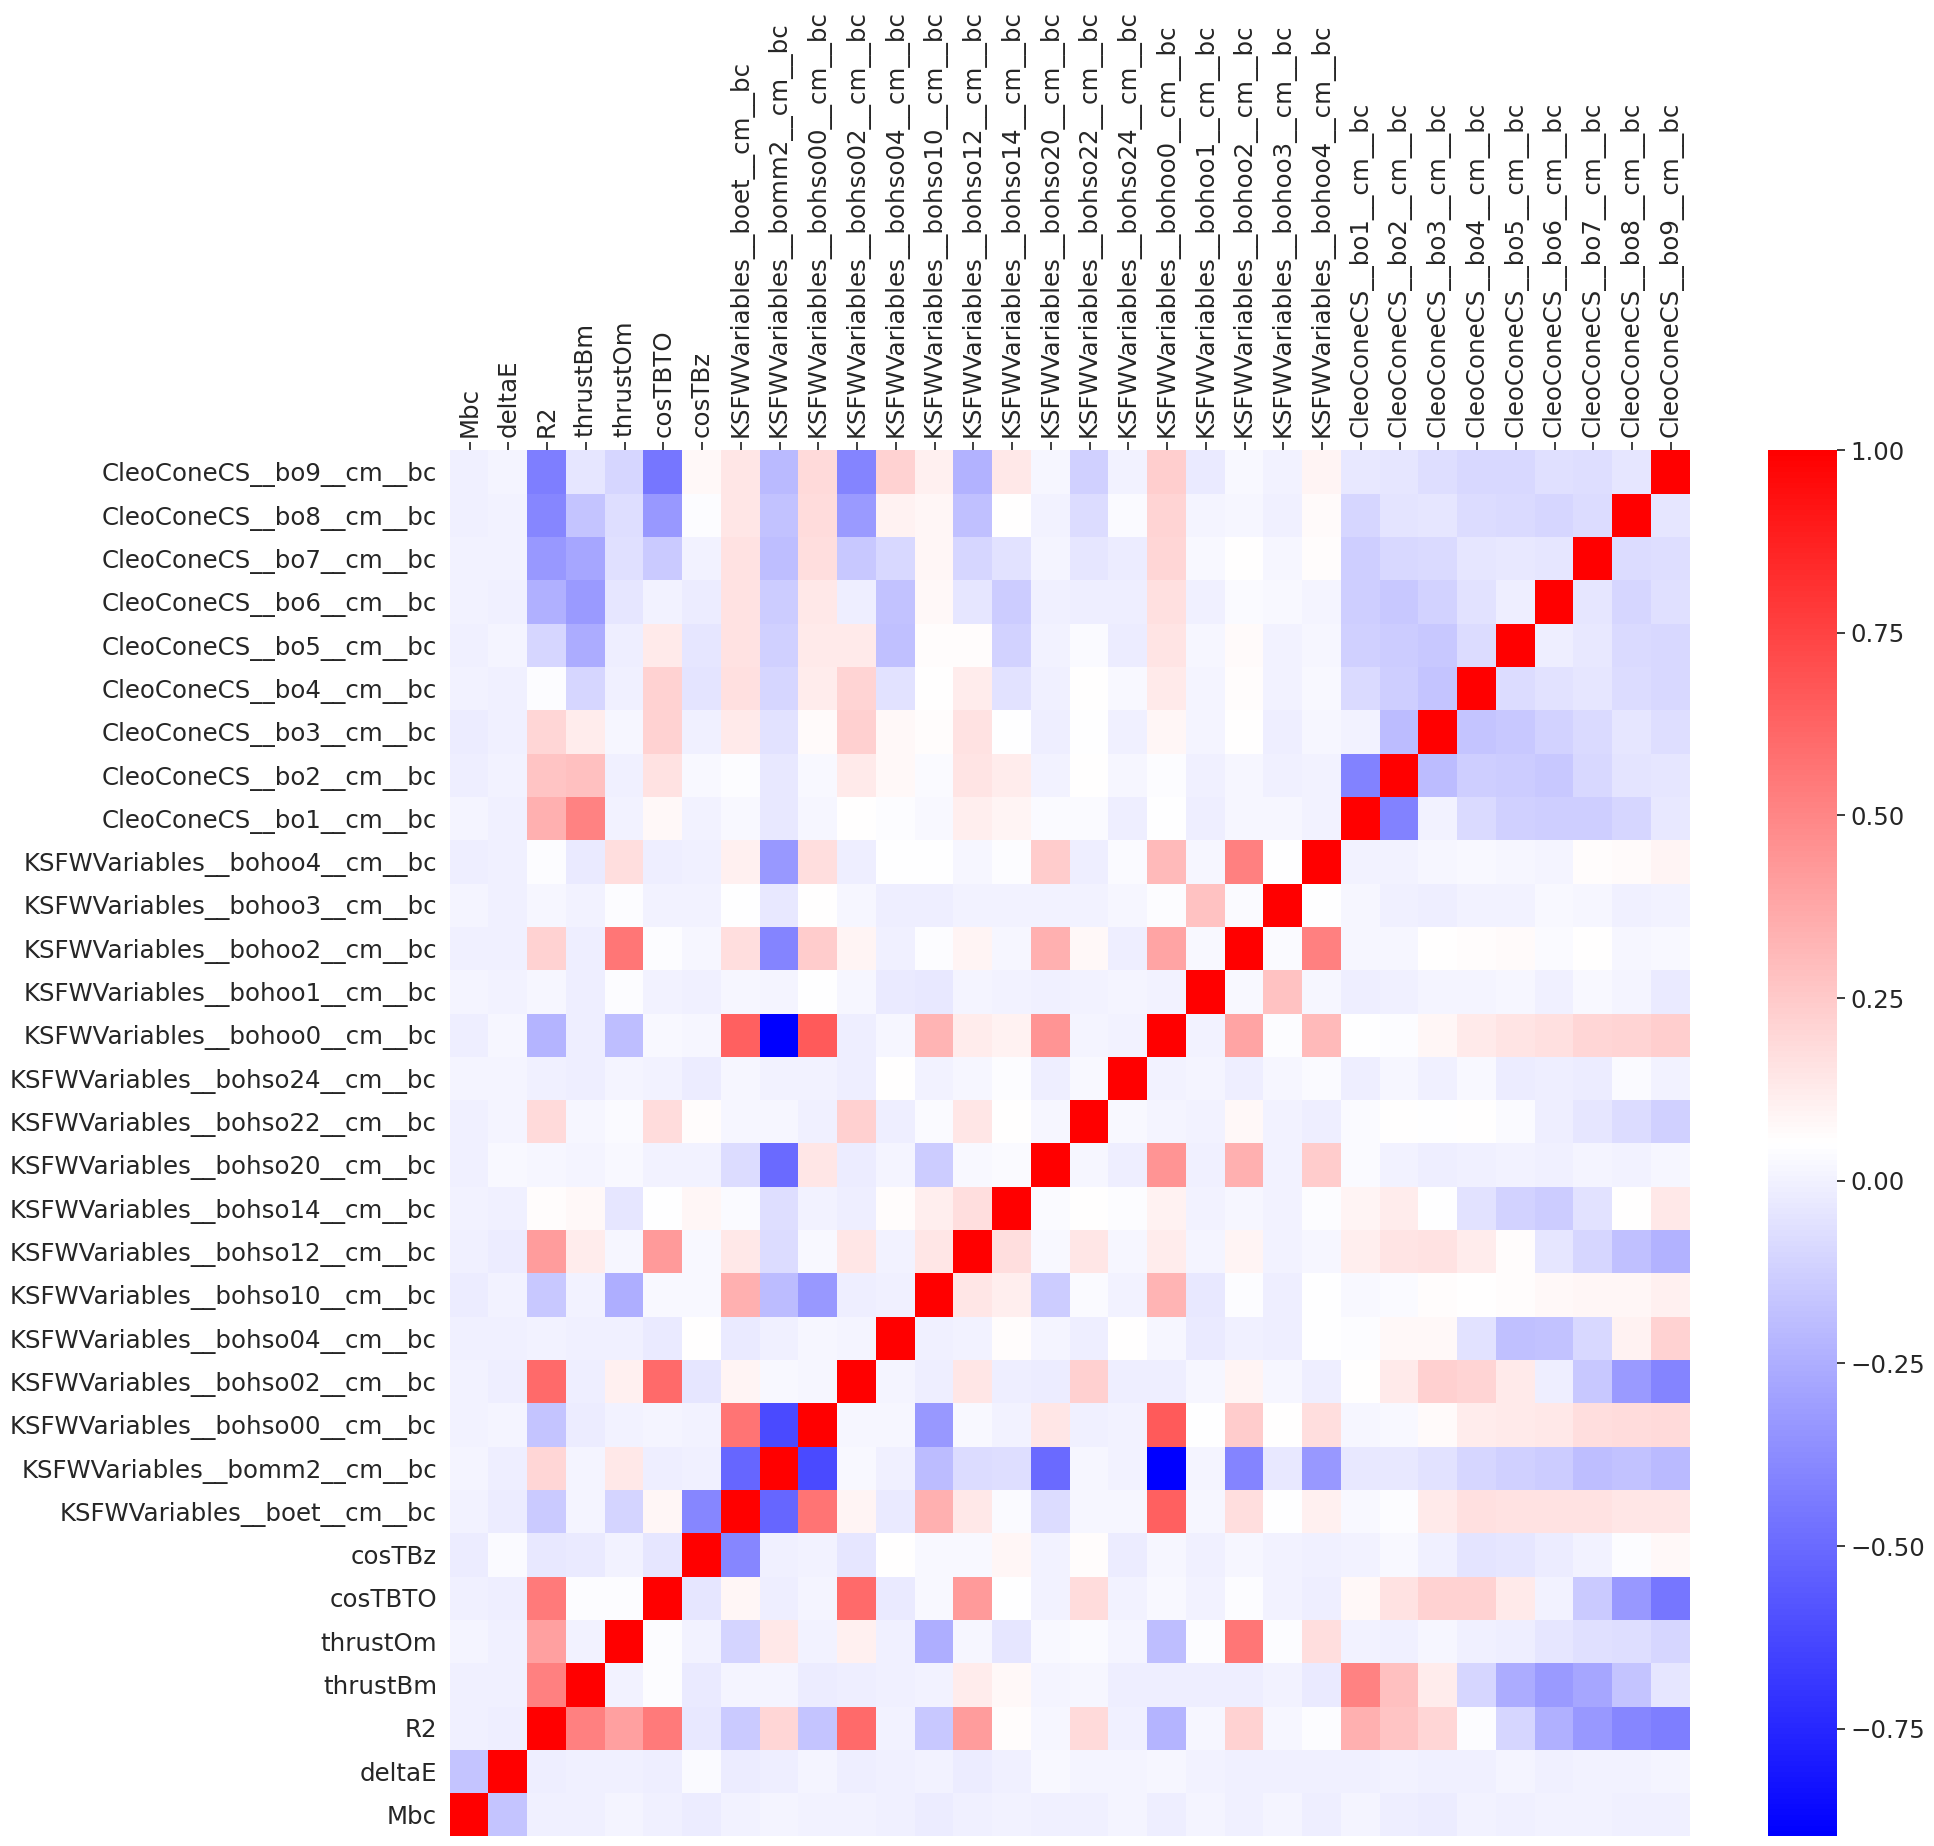
\includegraphics[width=1\linewidth]{figures/corr_cs_kine_sig}	
	\end{minipage}
\begin{minipage}[b]{0.5\linewidth}
	\centering 
	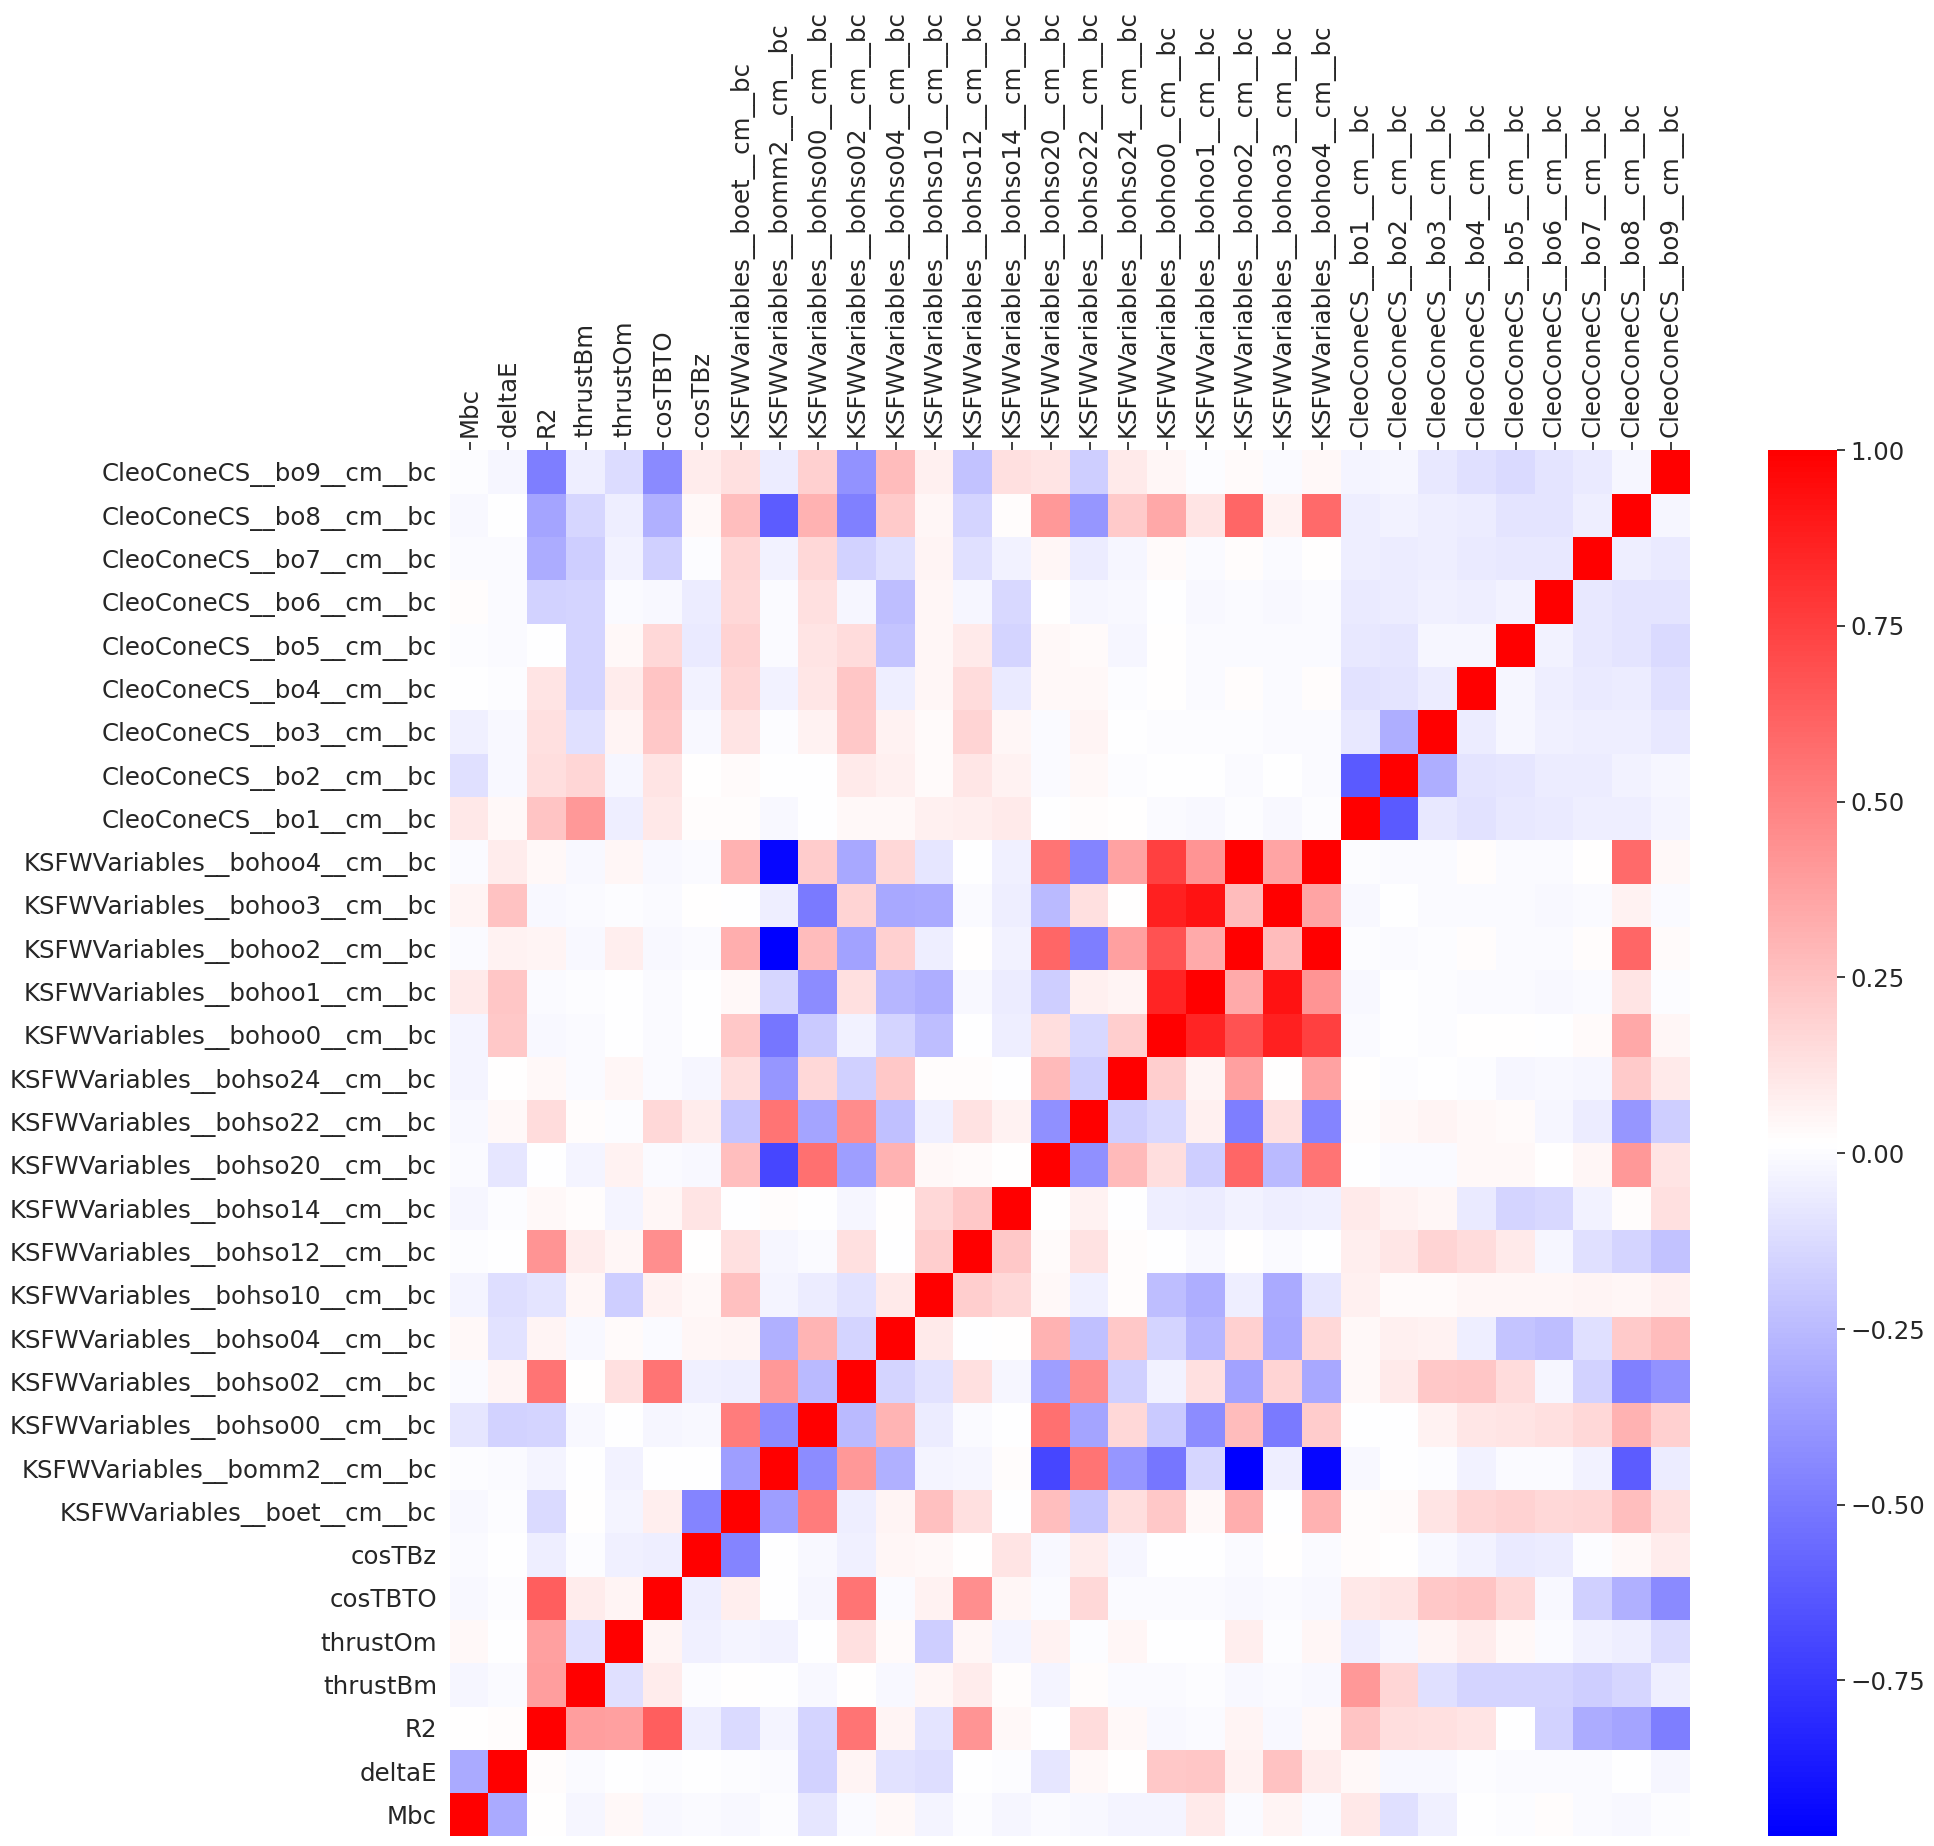
\includegraphics[width=1\linewidth]{figures/corr_cs_kine_bkg}	
\end{minipage}
	\caption{The correlation in variables for continuum suppression. The left is for signal and the right is for background.}
	\label{fig:cs_cor}
\end{figure}
\begin{figure}[htpb]
	\begin{minipage}[b]{0.5\linewidth}
		\centering 
		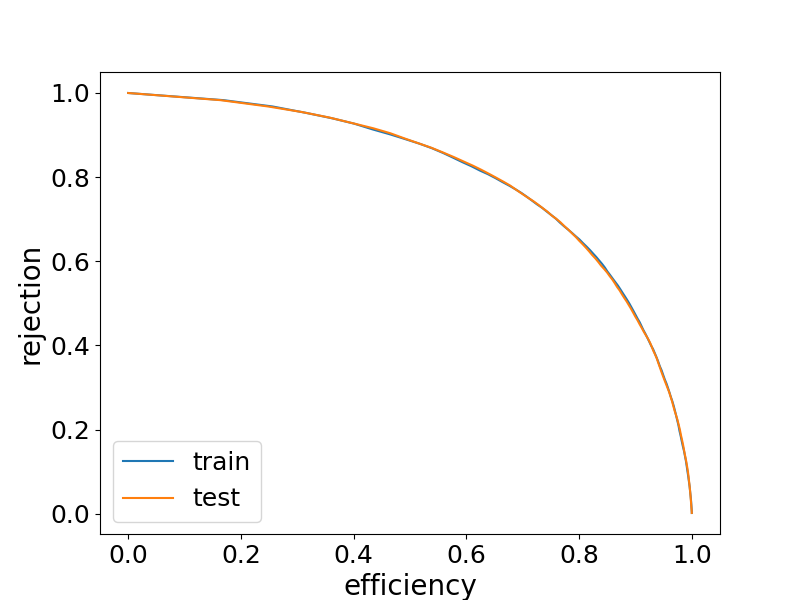
\includegraphics[height=6cm]{figures/ROC_CS}	
	\end{minipage}
	\begin{minipage}[b]{0.5\linewidth}
		\centering 
		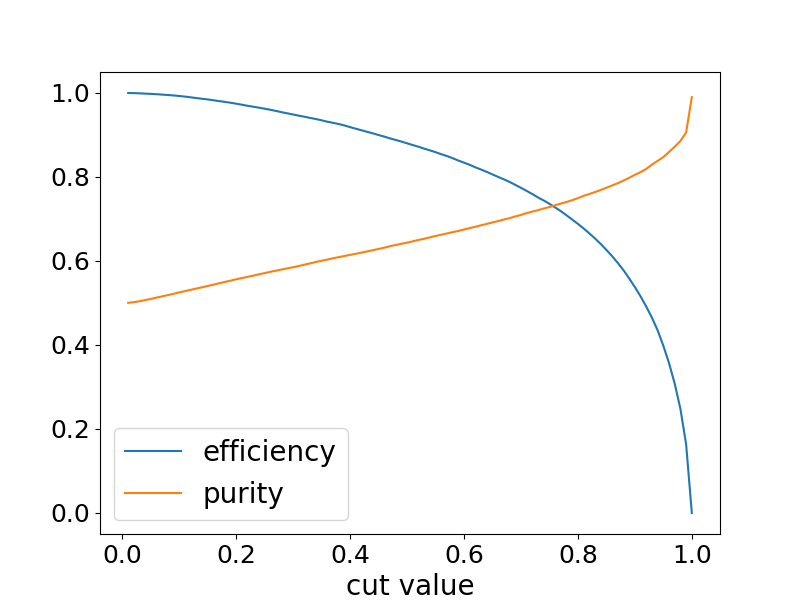
\includegraphics[height=6cm]{figures/eff_CS}	
	\end{minipage}
\caption{The left is the ROC curve (blue for training and orange for testing)
	and the right is the efficiency(blue) and purity(orange) regarding the classifier output \textit{FBDT\_CS}.}
	\label{fig:cs_roc}
\end{figure}

The Overtraining check is made by comparing the distribution of signal and background depending on the classifier output in both training and testing samples. The testing samples show about 1\% lower in each bin for both signal and background events, which is within the acceptable range.  
\begin{figure}[htpb]
	\centering
	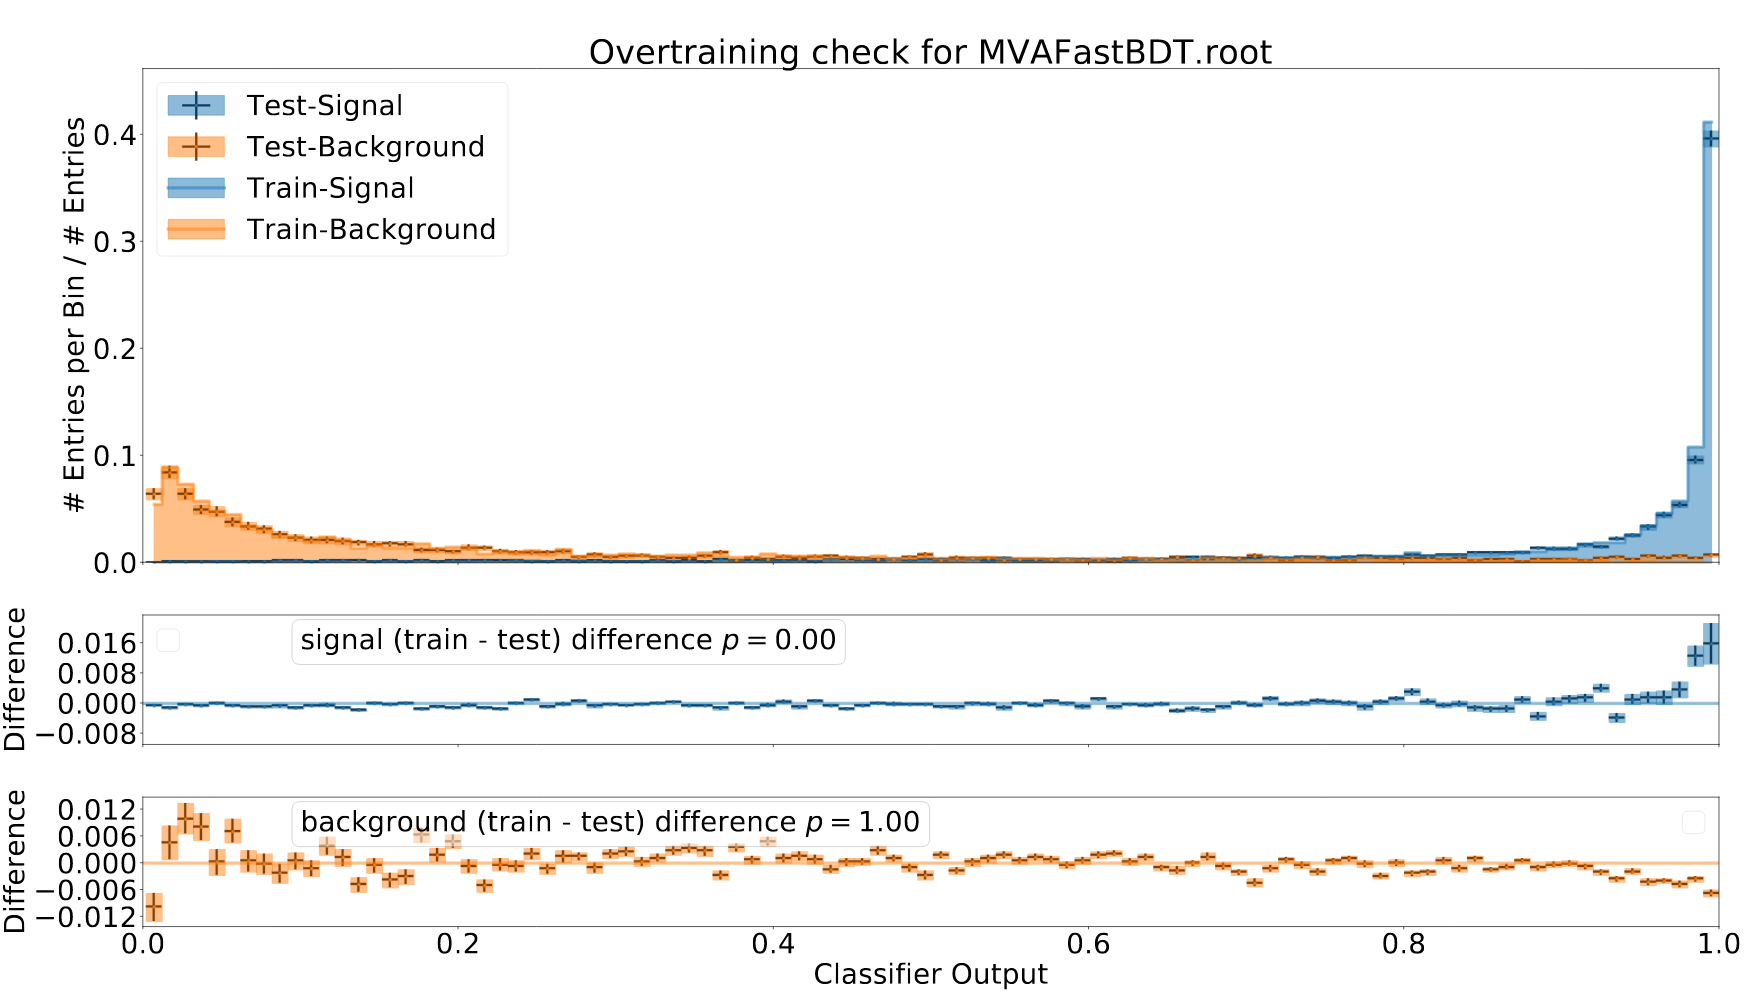
\includegraphics[width=1\linewidth]{cs-overtrain}
	\caption{Over-training check of continuum classifier, where a very small difference in training and testing (1\%) is shown.}
\end{figure}


\subsection{Event selection summary}
The summary of Event selections is listed in Table \ref{tab:b0select}, including the application of \textit{KsFinder} (by \textit{FBDT\_Ks}) and continuum suppression (by \textit{FBDT\_CS}).
\begin{table}[htpb]
	\centering 
	\begin{tabular}{c|c|c|c|c|c|c|c} 
		\hline
		$B^0$  & $M_{bc}$(GeV/$c^2$)& $\Delta E$(GeV) & $P(\chi^2)$ & \textit{Rank} & \textit{FBDT\_CS} & \textit{FBDT\_Ks}\\
		\hline
		Criteria & $> 5.20$ \& $< 5.29$  &  $ |\Delta E|< 0.2$ & $> 0.001$  & $=1$ & $>0.66$ & $>0.74$\\
		\hline
	\end{tabular}
	\caption{$B^0$ selection criteria, $P(\chi^2)$ is from $B^0$ $\it{CP}$-side vertex fit and \textit{Rank} is from the BCS}
	\label{tab:b0select}
\end{table}

Combined with the previous paragraph, the reconstruction performance of $B^0$ is summarized in Table \ref{tab:b0stats}. The efficiency, purity, fraction of multiplicity events and best candidates fraction of $B^0$ are slightly improved in the Belle II compared to the ones referenced from Belle.
\begin{table}[H]
	\centering
	\begin{tabular}{c|c|c|c|c}
		\hline
		event selection & efficiency & purity  & $f_{MB}$  & BCS \\
		\hline
		\hline
		Belle Standard & 35\%(33\%) & 96\%(99\%) & 6\%(6\%) & 83\%(96\%)\\
		\hline 
		Belle II (\textit{BG1}) & 36\%(34\%) & 96\%(98\%) & 4\%(4\%) & 95\%(96\%)\\
		\hline
		Belle II (\textit{BG0}) & 40\%(36\%) & 96\%(99\%) & 3\%(3\%) & 97\%(97\%)\\
		\hline
	\end{tabular}
	\caption{The efficiency is defined by the fraction of best candidates among the MC input number. Purity is the fraction of true $B^0$ in best candidates. $f_{MB}$ stands for multiple $B^0$ events fraction in true signal events. BCS is the fraction of best candidates being a true signal. All values in the parenthesis are calculated in $| M_{bc} |- 5.28 < 0.1$ and $|\Delta E| < 0.1$, called as ``signal region" where efficiency is lower but purity is higher, compared to the full range of $M_{bc}$ and $\Delta E$ in Table \ref{tab:b0select}. }
	\label{tab:b0stats}
\end{table}


% summary of $B^0$ stats goes here
\section{Resonance Background}

The $\it{CP}$ eigenvalue of $B^0 \to K_S^0  K_S^0  K_S^0$ is $\eta_f = +1$ if it is a loop-level $b\to s$ transition, called $\it{CP}$-even. However, the charmonium resonances from $b \to c$ tree-level transition can give an odd $\textit{CP}$ eigenvalue ($\eta_f = -1$) while producing the same final states as $B^0 \to K_S^0  K_S^0  K_S^0$.  This would cause the contamination to the $\it{CP}$ measurement due to the fact that $\mathcal{S} = -\eta_f\text{sin}(2\phi_1)$. The loop-level $\it{CP}$-even processes are demonstrated in the left and middle diagrams of Figure \ref{fig:3ksfey}, including the phase-space based decay and resonance decays. Both are considered as the signal events. The tree-level $\it{CP}$-odd process is shown in the right diagram of Figure \ref{fig:3ksfey}, which is usually referred as the resonance background and can be rejected by applying cut on the invariant mass of two $K_S^0$ around the possible charmonium resonant states. Therefore, to check wether a resonance decay is a signal or background event, a list of possible $B^0 \to X(\to K^0_S K^0_S) K^0_S$ processes are considered. For the resonance decays of signal events, $X$ could be $f_2(1270)$, $f_0(1500)$, $f_{2}^{'}(1525)$, $f_0(980)$, $f_0(1710)$ and $f_2(2010)$. For resonance background, \textit{X} could be $D^0$, $J/\psi$, $\psi(2S)$,  $\chi_{c0}$, $\chi_{c1}$, and $\chi_{c2}$.
The branching fraction of these decay modes in the PDG and the Belle II decay profile are both checked and compared, where some of them are not yet measured or not implemented in the Belle II simulation. Thus it is hard to precisely evaluate all the contributions from these decay modes. The expected contributions are calculated by using $2.14\times 10^8 B\bar{B}$ pairs as shown in the Table \ref{tab:f_res}. The main contribution from the resonance background is $B^0\to \chi_{c0} K^0_S$ and the main contribution from the resonant signal is $B^0\to f_0(980)K^0_S$. Given the very limited statistics of data accumulation we used in this analysis, the contribution of $\it{CP}$-odd resonance background should be smaller than one event. Besides, the comparison of two $K_S^0$ invariant mass using data and \textit{generic MC} is performed, while the small number of reconstructed events in data can not provide reasonable information on the distribution, see Appendix C. Hence, currently there is no veto of two $K_S^0$ invariant mass is applied to avoid potential bias in this low statistics scenario. In the future with more data collected, the veto will be first checked by the proper comparison between data and MC, then applied according to mass of the main contributive resonance states.
\begin{sidewaystable}
	\caption{Expected yield for signal and background resonances $2.14\times 10^8 B\bar{B}$ in \textit{generic MC}. The branching fraction of $B\to X K_S$ and $X \to 2K_S$ are listed from both the PDG values and the values used in Belle II generic decay profile. The number of events from $\it{CP}$-odd resonance background is expected to be smaller than one at current luminosity 62.8 fb$^{-1}$.}
	\label{tab:f_res}
	\centering
	\begin{tabular}{|c|c|c|c|c|c|c|}
		\hline
		Resonances & Br($B \to X K_S$)PDG  & Br($X \to2K_S$) & Br($B \to X K_S$)Dec. & Br($X \to2K_S$)Dec. & $B\bar{B}$ pairs & Expected yields \\
		\hline
		$D^0 K_S$ & $2.6 \times 10^{-5}$ & $1.7\times 10^{-4}$ & $2.6 \times 10^{-5}$ & $1.8\times 10^{-4}$ & $2.14\times 10^8$ & 0.134 \\
		\hline
		$\eta K_S$ & $3.45\times 10^{-4}$ & $<3.1\times 10^{-4}$ & $4\times 10^{-4}$ & No Value & $2.14\times 10^8$ & No Value  \\
		\hline
		$J/\psi K_S$ & $4.35\times 10^{-4}$ & $<1.4\times 10^{-8}$ & $4.35\times 10^{-4}$ & 0 & $2.14\times 10^8$ & 0 \\
		\hline
		$\psi(2S)K_S$ & $2.9\times 10^{-4}$ & $<4.6\times 10^{-6}$ & $2.9\times 10^{-4}$ & 0 & $2.14\times 10^8$ & 0 \\
		\hline
		$\chi_{c0}K_S$ & $7.3\times 10^{-5}$ & $3.16\times 10^{-3}$ & $7.35\times 10^{-5}$ & $3.1\times 10^{-3}$ & $2.14\times 10^8$ & 6.21 \\
		\hline
		$\chi_{c1}K_S$ & $1.96\times 10^{-4}$ & $6\times 10^{-5}$ & $1.96\times 10^{-4}$ & $1\times 10^{-5}$ & $2.14\times 10^8$ & 0.05 \\
		\hline
		$\chi_{c2}K_S$ & $7.5\times 10^{-6}$ & $2.6\times 10^{-4}$ & $7.5\times 10^{-6}$ & $5.5\times 10^{}-4$ & $2.14\times 10^8$ & 0.11 \\
		\hline
		$f_2(1270)K_S$ & $1.35\times 10^{-6}$ & $1.15\times 10^{-2}$ & $1.35\times 10^{-6}$ & $1.15\times 10^{-2}$ & $2.14\times 10^8$ & 0.42 \\
		\hline
		$f_{2}^{'}(1525)K_S$ & $1.5\times 10^{-7} $ & $2.22\times 10^{-2}$ & No value & 0.22 & $2.14\times 10^8$ & No Value \\
		\hline
		$f_2(2010)K_S$ & $5\times 10^{-7}$ & No Value  & No Value  & No Value  & $2.14\times 10^8$ & No Value \\
		\hline
		$f_0(980)K_S$ & $2.7\times 10^{-6}$ & No Value & $2.75\times 10^{-6}$ & No Value & $2.14\times 10^8$ & 43.3 \\
		\hline
		$f_0(1710)K_S$ & $5\times 10^{-7}$ & No Value  & No Value  & No Value  & $2.14\times 10^8$ & No Value \\
		\hline
		$f_0(1500)K_S$ & $6.5\times 10^{-5}$ & 0.022 & No Value & 0.022 & $2.14\times 10^8$ & No Value \\
		\hline
		Total  & - & - & - & - & - & $\simeq$50 \\
		\hline
	\end{tabular}
\end{sidewaystable}


% 2021.02.10 mid
\section{$B\bar{B}$ background}
Another possible contribution of background comes from $B\bar{B}$ events. Both neutral and charged $B\bar{B}$ pairs could produce the background events. Compared to the event number from the continuum background, the number of $B\bar{B}$ background is much fewer. By counting the background event number from $B\bar{B}$ and $q\bar{q}$ using \textit{generic MC}, the fraction of $B\bar{B}$ takes about 3\% among all background events, and no special treatment is implemented. 

\section{Signal Extraction}
The event selections defined in Table \ref{tab:b0select} is applied to \textit{signal MC}, \textit{generic MC} and experiment data for extracting signal events. The integral luminosity in \textit{generic MC} is 1 ab$^{-1}$ and experiment data used in this analysis is 62.8 fb$^{-1}$ from the latest official processing. The distribution of $M_{bc}$ and $\Delta E$ from \textit{generic MC} are shown in Figure \ref{fig:2Dgenstack} which contains 328 signal events,  702 continuum background events and 35 $B\bar{B}$ background events. The distribution of $M_{bc}$ and $\Delta E$ from data are also shown in Figure \ref{fig:2Dgenstack}.

\begin{figure}[htpb]
	\begin{minipage}[b]{0.5\linewidth}
		\centering 
		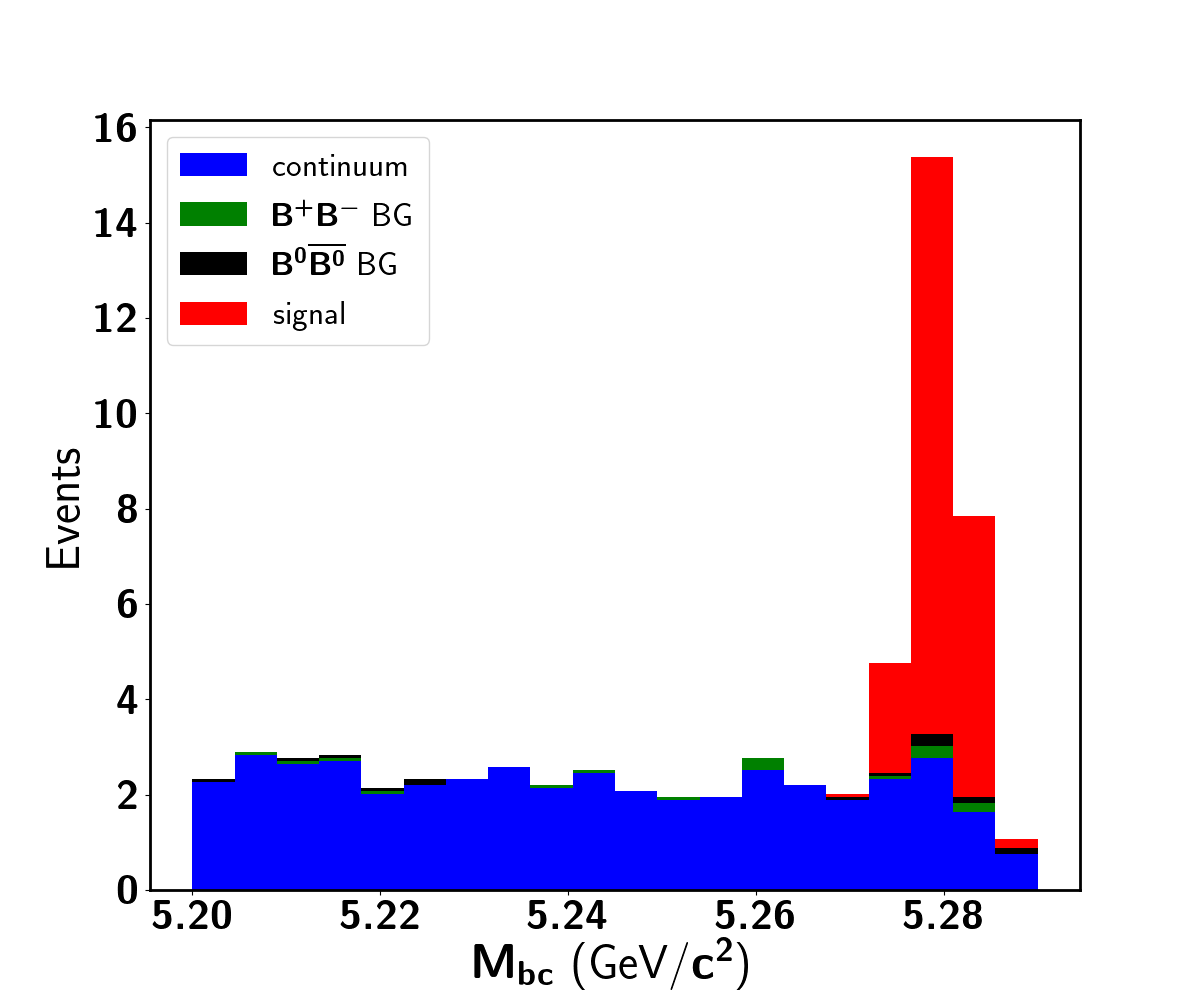
\includegraphics[width=1\linewidth]{figures/hist_stacked_generic_mbc_oldksfinder}
	\end{minipage}
	\begin{minipage}[b]{0.5\linewidth}
		\centering 
		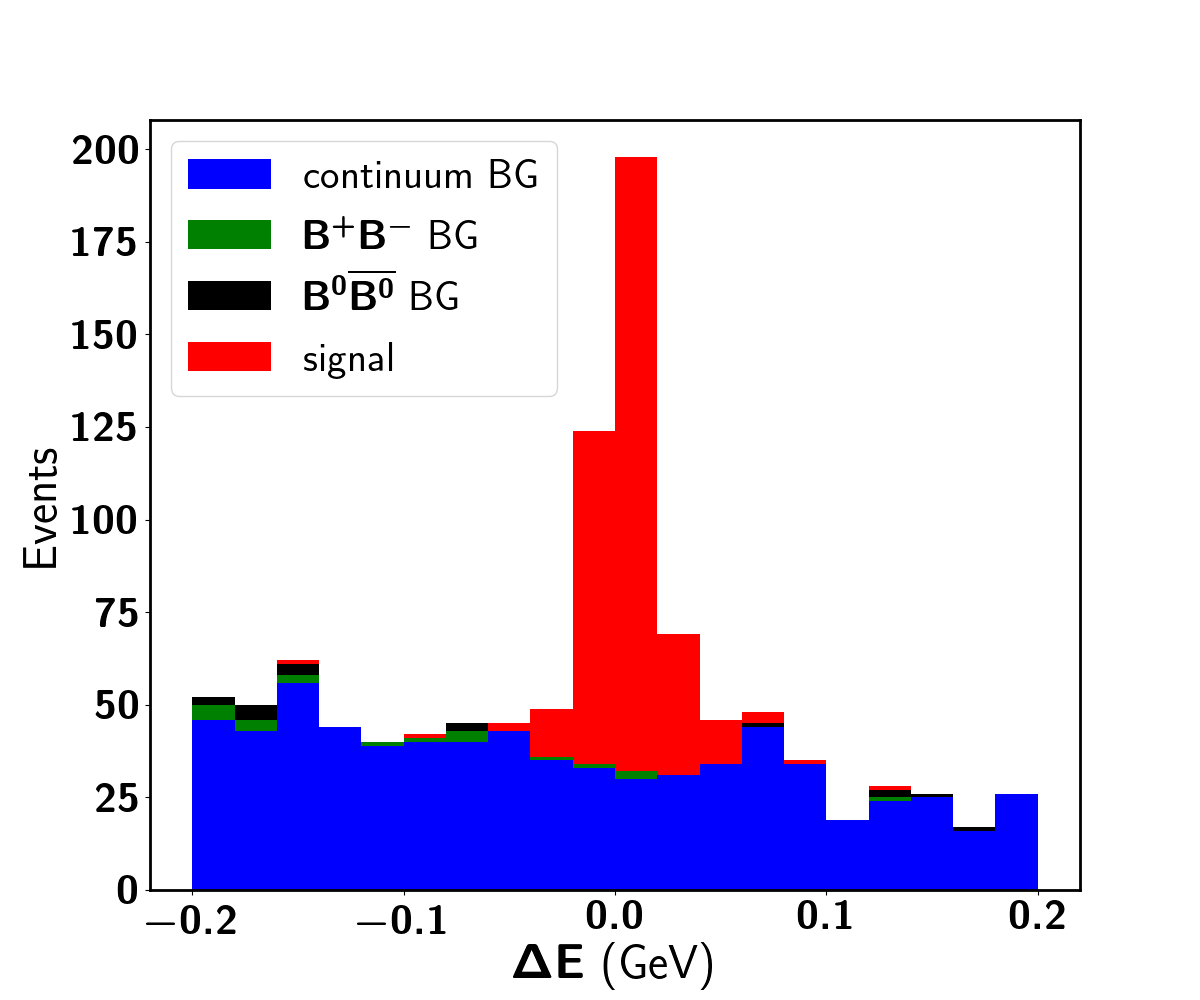
\includegraphics[width=1\linewidth]{figures/hist_stacked_generic_dE_oldksfinder}
	\end{minipage}
	\caption{The distribution  of $M_{bc}$ and $\Delta E$ for selected events from \textit{generic MC}, where each background components are stacked with signal. The blue component is the continuum background. The green and the black are the background from charged and neutral $B\bar{B}$ events. The red component is the signal component by checking MC truth matching. }
	\label{fig:2Dgenstack}
\end{figure}
\begin{figure}[H]
	\begin{minipage}[b]{0.5\linewidth}
		\centering 
		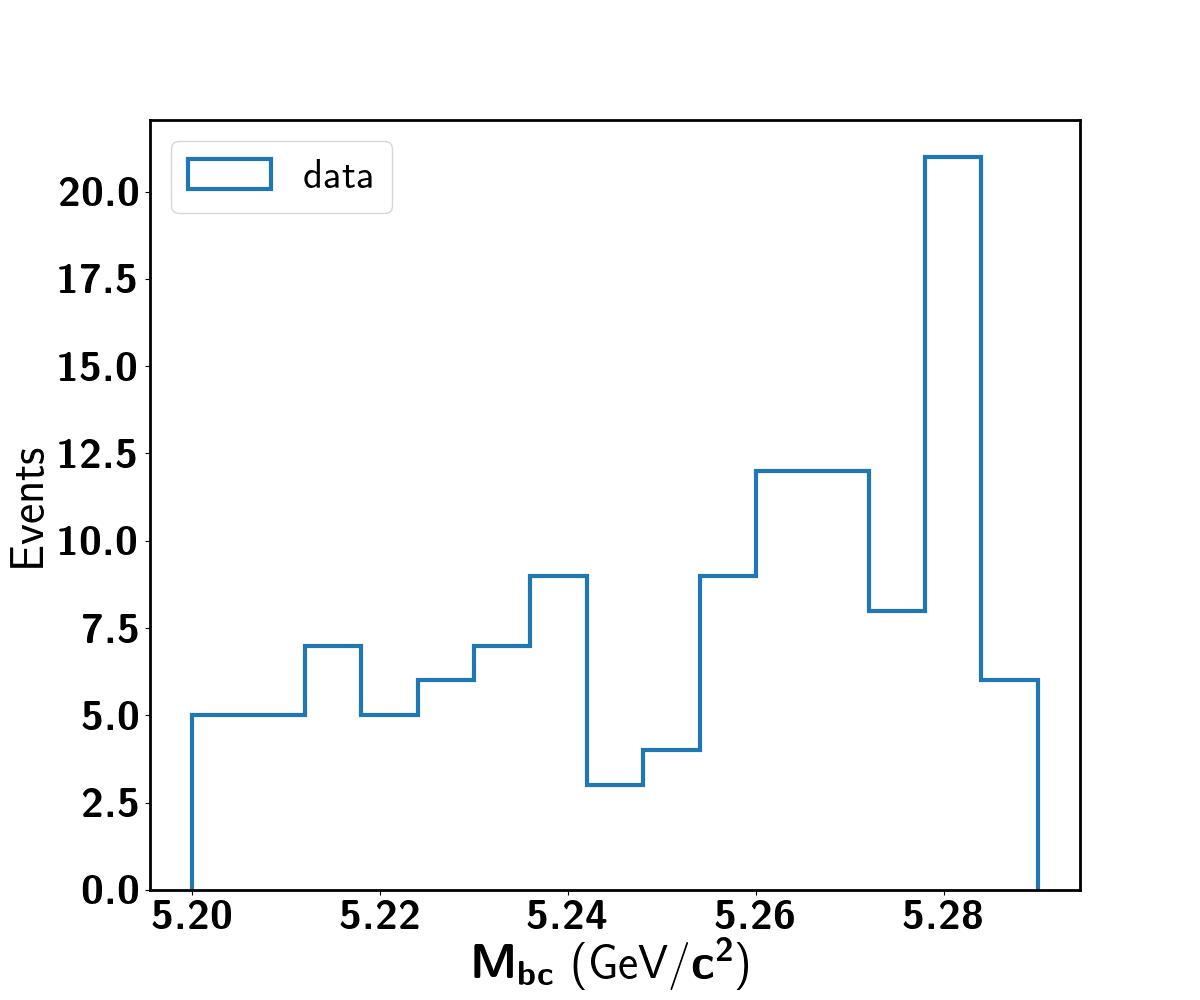
\includegraphics[width=1\linewidth]{figures/hist_stacked_data_mbc_ksfinder}
		\label{}
	\end{minipage}
	\begin{minipage}[b]{0.5\linewidth}
		\centering 
		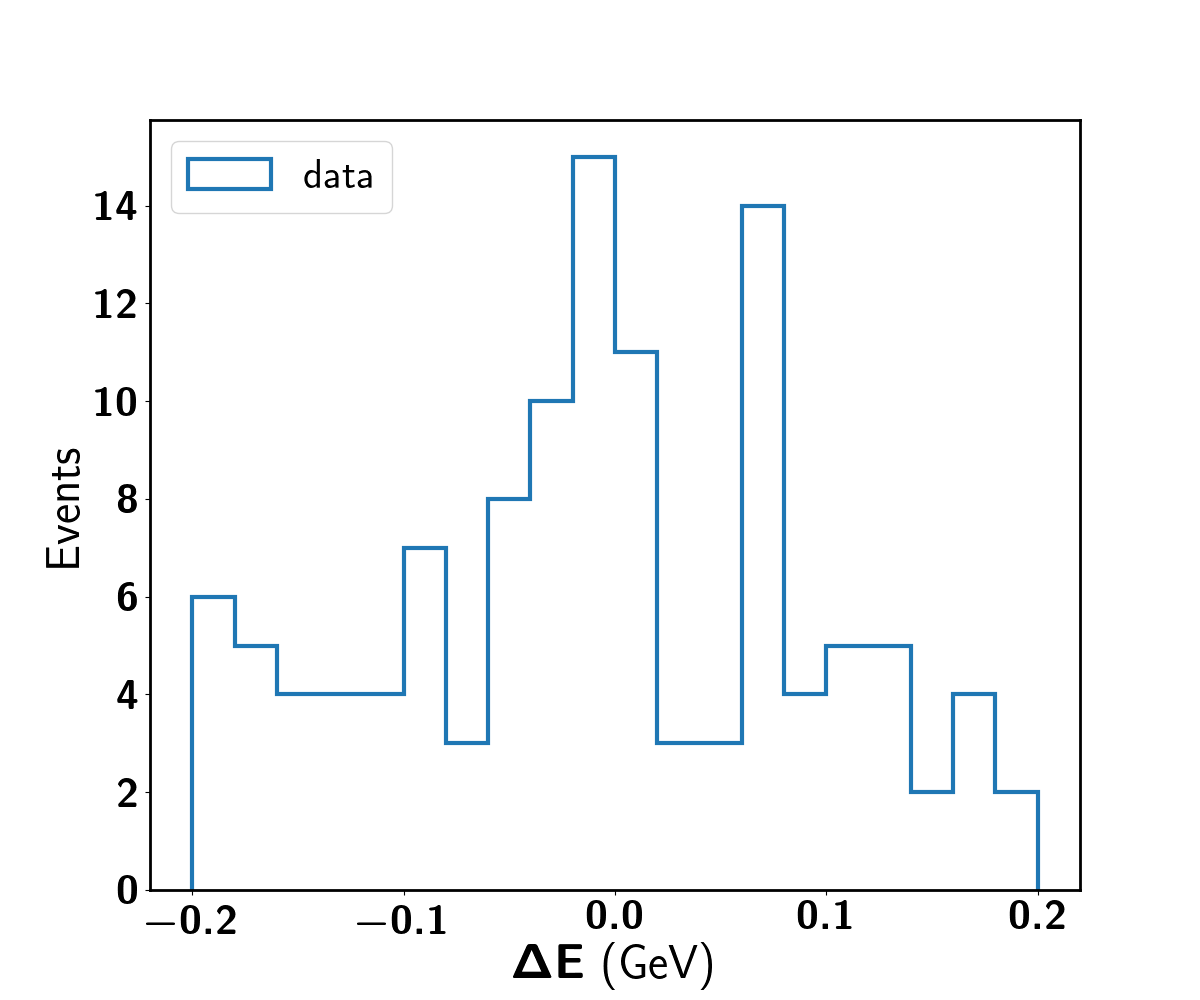
\includegraphics[width=1\linewidth]{figures/hist_stacked_data_dE_ksfinder}
		\label{}
	\end{minipage}
	\caption{The distribution  of $M_{bc}$ and $\Delta E$ for selected events from data.}
	\label{fig:2Ddatastack}
\end{figure}

The unbinned maximum likelihood fit using RooFit is performed to extract the signal. The 2D fit using both $M_{bc}$ and $\Delta{E}$ are done by taking the probability density function:
\begin{equation}\label{eq:pmbcde}
\mathcal{P}(M_{bc},\Delta{E}) = 
f_{sig}\times \mathcal{P}_{sig}^{M_{bc}}\times\mathcal{P}_{sig}^{\Delta{E}}
+ 
(1-f_{sig})\mathcal{P}_{bkg}^{M_{bc}}\times\mathcal{P}_{bkg}^{\Delta{E}} ~,
\end{equation}
where $\mathcal{P}_{sig}^{M_{bc}}$ and $\mathcal{P}_{sig}^{\Delta{E}}$ are the probability density function (P.D.F) for the distributions of $M_{bc}$ and $\Delta E$. The $f_{sig}$ is the fraction of signal events. We use the single Gaussian function as $\mathcal{P}_{sig}^{M_{bc}}$  in the distribution of $M_{bc}$ and triple Gaussian functions as $\mathcal{P}_{sig}^{\Delta{E}}$  in the distribution of $\Delta E$ to model the signal component. 

On the other hand, the dominated background comes from the continuum events, which is modeled as the Argus distribution~\cite{albrecht1990search} in the distribution of $M_{bc}$:
\begin{equation}\label{eq:Argus}
\mathcal{P}_{bkg}^{M_{bc}}(x;c,\chi)=\frac{\chi^3}{\sqrt{2\pi}\Psi(\chi)}\cdot
\frac{x}{c^2}\sqrt{1-\frac{x^2}{c^2}}\cdot
\exp \begin{Bmatrix}
-\frac{1}{2}\chi^2(1-\frac{x^2}{c^2}) ~
\end{Bmatrix}~,
\end{equation}
where $x$ presenting $M_{bc}$ is defined in $0<x<c$ with a preset mass threshold at $c = 5.29$ GeV. The $\chi$ is  parameter of the distribution. The $\Psi(\chi)=\Phi(\chi)-\chi\phi(\chi)-\frac{1}{2}$ where $\Phi(\chi)$ and $\phi(\chi)$ are cumulative distribution and probability density function of the standard normal distribution, respectively. The $\Delta E$ distribution of continuum events is modeled by the first order Chebyshev polynomial function.

The unbinned maximum likelihood fit is first performed to obtain the parameters for signal functions using \textit{signal MC}, and then fixed them as the constants latter for 2D fit. The fit results on \textit{signal MC} are shown in Figure \ref{fig:mbcde1D}. The continuum background is fitted by using $q\bar{q}$ events from \textit{generic MC} to determine the shapes then fix them as the constants latter for 2D fit. The fit results on \textit{$q\bar{q}$} events are shown in Figure \ref{fig:bkgmbcde}.
 \begin{figure}[htbp]
 	\begin{minipage}[b]{0.5\linewidth}
 		\centering 
 		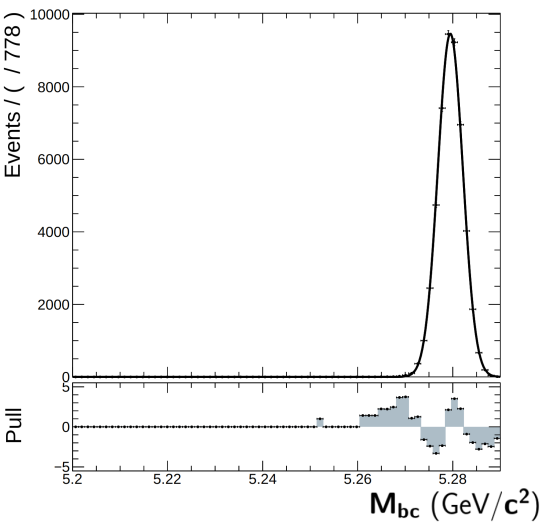
\includegraphics[height=6cm]{mbc_sig_fit}
 		%\label{fig:side:a}
 	\end{minipage}
 	\begin{minipage}[b]{0.5\linewidth}
 		\centering 
 		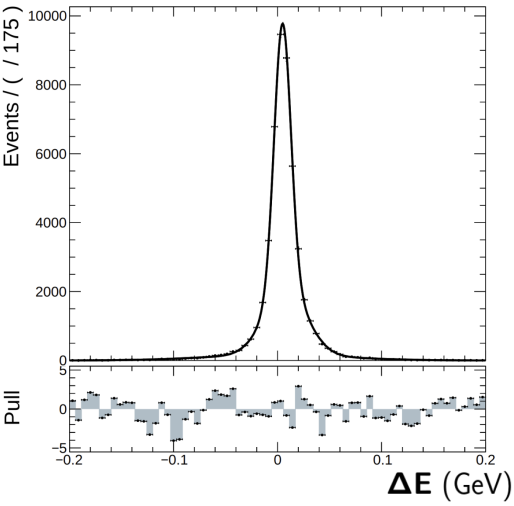
\includegraphics[height=6cm]{de_sig_fit}
 		%\label{fig:side:b}
 	\end{minipage}
 	\caption{The distribution of $M_{bc}$ and $\Delta E$ of \textit{signal MC} of $B^0 \to K_S^0  K_S^0  K_S^0$ fitted with single and triple Gaussian functions respectively. The bottom plots are the pull of the data points and the fit result.}
 	\label{fig:mbcde1D}
 \end{figure}
\begin{figure}[htbp]
	\begin{minipage}[b]{0.5\linewidth}
		\centering 
		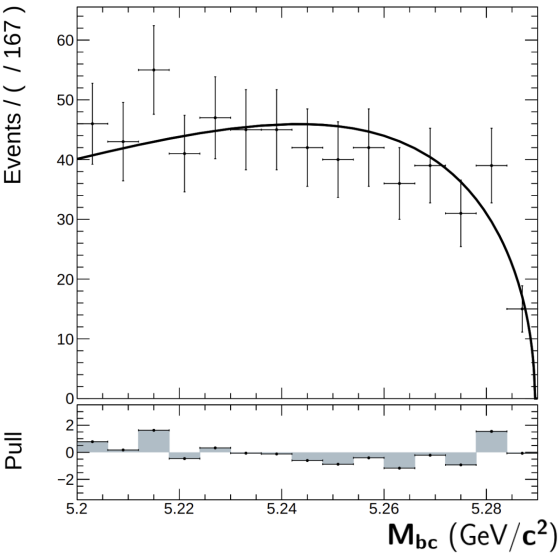
\includegraphics[height=6cm]{figures/mbc_cs_fit}
		\label{}
	\end{minipage}
	\begin{minipage}[b]{0.5\linewidth}
		\centering 
		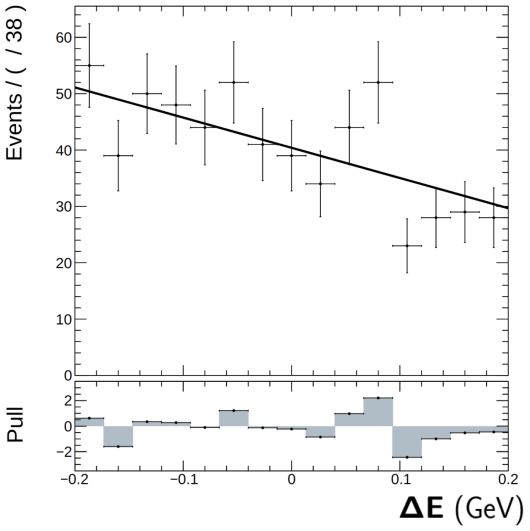
\includegraphics[height=6cm]{figures/de_cs_fit}
		\label{}
	\end{minipage}
	\caption{The distribution of $M_{bc}$ and $\Delta E$ of continuum events in \textit{generic MC} fitted with Argus and Chebyshev polynomial functions, respectively.  The bottom plots are the pull of the data points and the fit result.}
	\label{fig:bkgmbcde}
\end{figure}

Then we set the events number for signal and background as floating parameters and use Equation \ref{eq:pmbcde} as the 2D model to fit on 1 ab$^{-1}$ \textit{generic MC} as shown in the Figure \ref{fig:2Dgen}.

\begin{figure}[htpb]
	\begin{minipage}[b]{0.5\linewidth}
		\centering 
		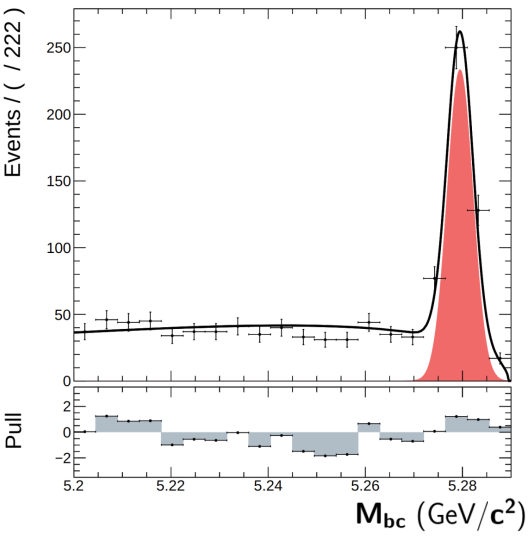
\includegraphics[height=6cm]{figures/mbc_data_fit}
		\label{}
	\end{minipage}
	\begin{minipage}[b]{0.5\linewidth}
		\centering 
		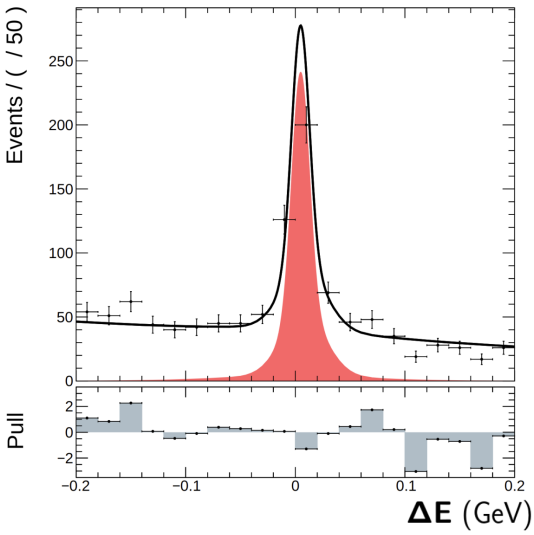
\includegraphics[height=6cm]{figures/de_data_fit}
		\label{}
	\end{minipage}
	\caption{Top is the stacked plots for \textit{generic MC} of $M_{bc}$ and $\Delta E$, where each background components are stacked with signal. The bottom is the 2D fit on 1 ab$^{-1}$ \textit{generic MC} projected on $M_{bc}$(GeV/$c^2$) and $\Delta E$(GeV), the red is signal component from the fit result in both plots.}
	\label{fig:2Dgen}
\end{figure}

Before perform 2D fit on experiment data, the distribution of $K_S^0$ invariant mass from the reconstructed $B^0$ candidates is compared between \textit{generic MC} and experiment data. The selection criteria in Table \ref{tab:b0select} are applied to both samples. The distributions are shown in Figure \ref{fig:b0ksmass}, where the \textit{generic MC} is scaled to the luminosity of experiment data and an agreement within $\sim 1\sigma$ is observed. 

\begin{figure}[htbp]
\begin{minipage}[b]{0.5\linewidth}
	\centering 
	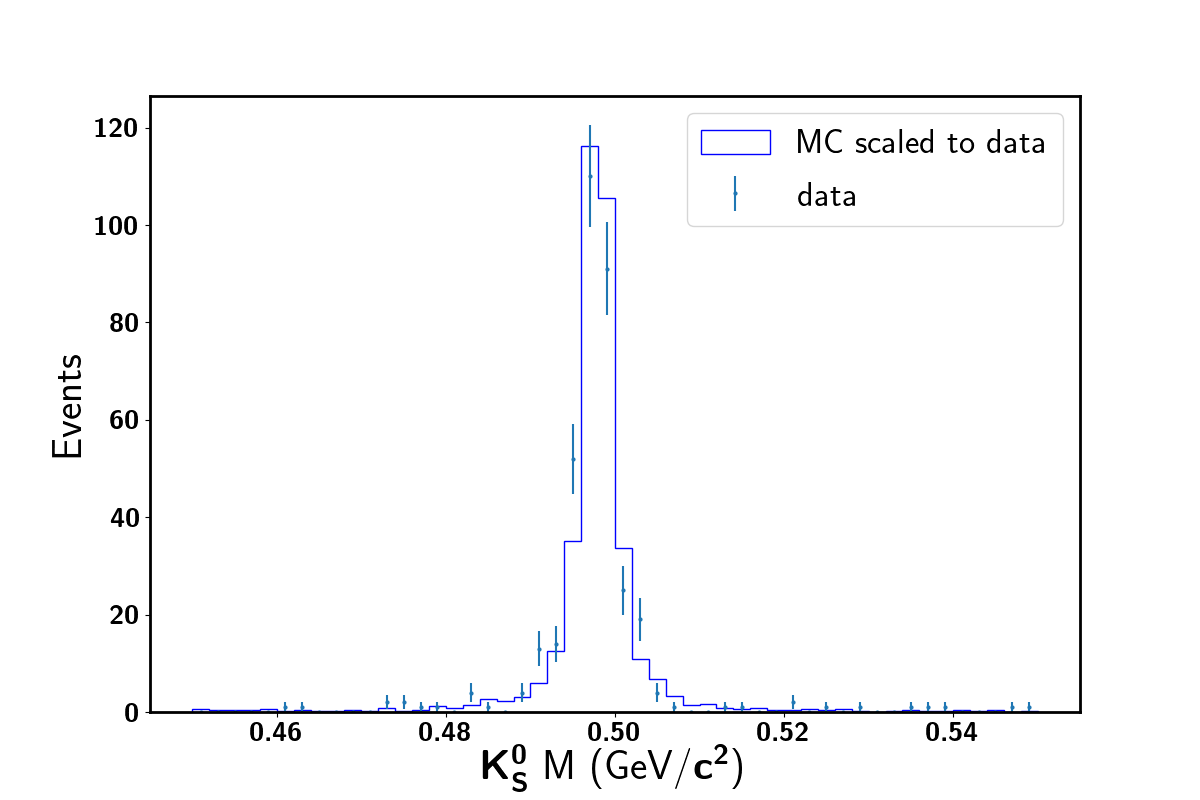
\includegraphics[width=1\linewidth]{figures/best_KsM}	
\end{minipage}
\begin{minipage}[b]{0.5\linewidth}
	\centering 
	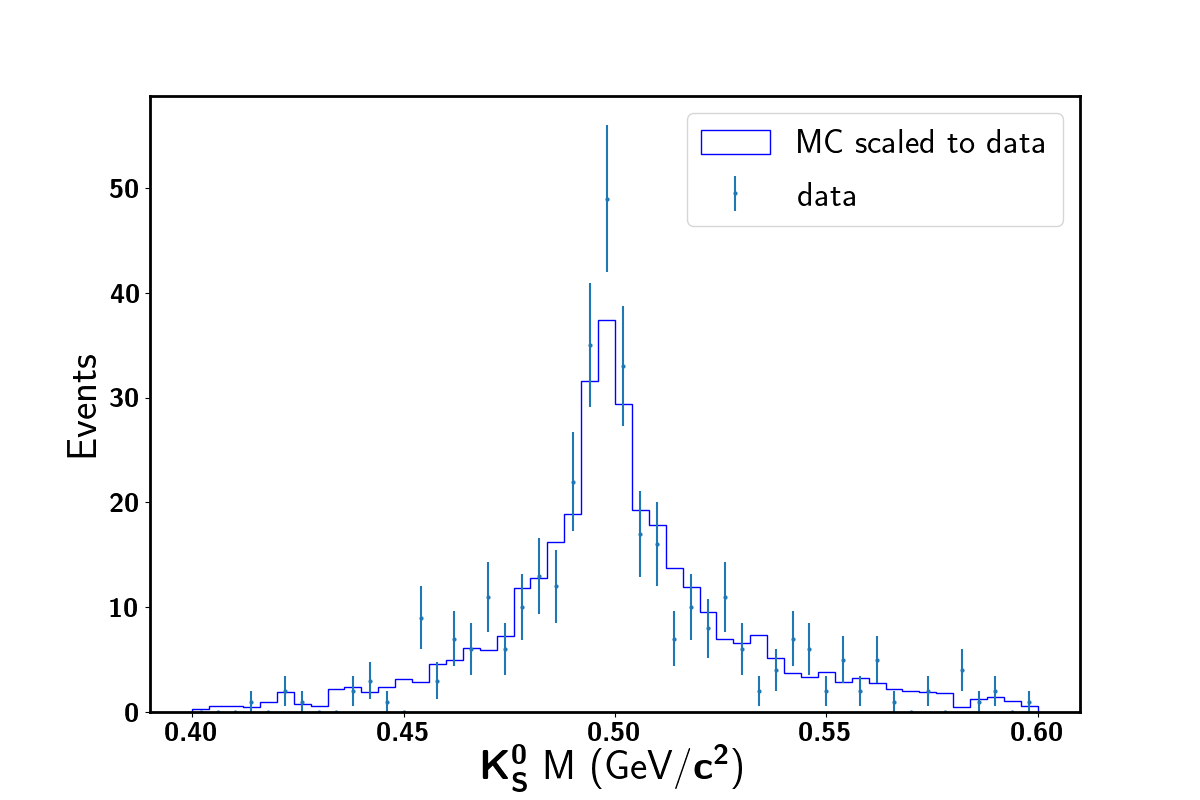
\includegraphics[width=1\linewidth]{figures/best_KsInvM}	
\end{minipage}
\caption{Invariant mass before (left) and after (right) $B^0$ vertex fit from \textit{generic MC} and experiment data.}
\label{fig:b0ksmass}
\end{figure}

\begin{figure}[htbp]
	\begin{minipage}[b]{0.5\linewidth}
		\centering 
		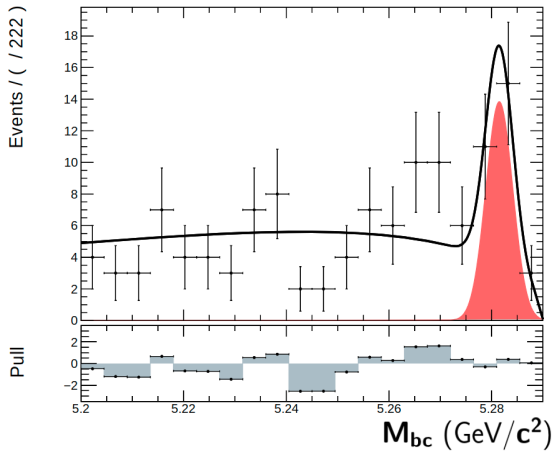
\includegraphics[height=5.8cm]{figures/mbc_2d_fit}
		\label{}
	\end{minipage}
	\begin{minipage}[b]{0.5\linewidth}
		\centering 
		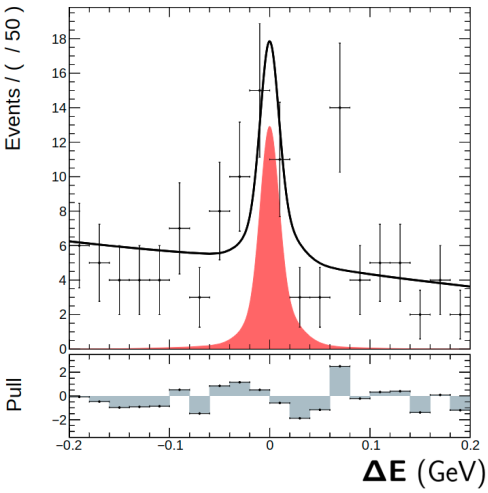
\includegraphics[height=5.8cm]{figures/de_2d_fit}
		\label{}
	\end{minipage}
\caption{$M_{bc}$(GeV) and $\Delta E$(GeV) 2D fit on 62.8 fb$^{-1}$data, the red is the signal component.}
\label{fig:2Ddata}
\end{figure}

Same as the fit procedure for the \textit{generic MC}, the 2D fit of the experiment data is done and the distributions projected on $M_{bc}$ and $\Delta E$ are shown in Figure \ref{fig:2Ddata}.  The number of signal events is extracted by the integral of fit model over the signal region which is defined as $5.27 < M_{bc} < 5.29 $ GeV and $-0.1 < \Delta E < 0.1$ GeV.
 Using Equation \ref{eq:b0nsig}:
 \begin{equation}\label{eq:b0nsig}
  {N_{sig}}=
\mathcal{B}(B^0 \to K_S^0  K_S^0  K_S^0) \times {\mathcal{B}(K_S^0\to \pi^+\pi^-)^3\times
 	\epsilon_{rec}\times N_{B\bar{B}}\times 2} ~,
 \end{equation}
the estimated signal event number can be calculated, where the $N_{B\bar{B}}$ is the number of neutral $B$ meson pairs calculated from the integrated luminosity and $\epsilon_{rec}$ is the reconstruction efficiency. The factor 2 accounts for the fact that both $B^0$ and $\overline{B^0}$ can decay to three $K_S^0$ in the final states.

\begin{comment}
In 1 ab$^{-1}$ \textit{generic MC}, the number of the expected signal events, where $\epsilon_{rec} = 34\%$ is taken from Table \ref{tab:b0stats}, is obtained by $7.7\times 10^8 \times 6\times 10^{-6} \times 21\% \times 34\% \simeq 329$. The 2D fit result from $M_{bc}$ and $\Delta E$ yields $341\pm 20$ events which agrees with expected number within $1\sigma$. The number of events in sideband defined as $M_{bc}<5.26$ GeV/$c^2$ in \textit{generic MC} is 507.
Using the Belle result with $772\times 10^6$ $B\overline{B}$ pairs, the number of signal events is estimated to be $327\pm 19$~\cite{kang2020measurement}.
\begin{figure}[htpb]
\centering
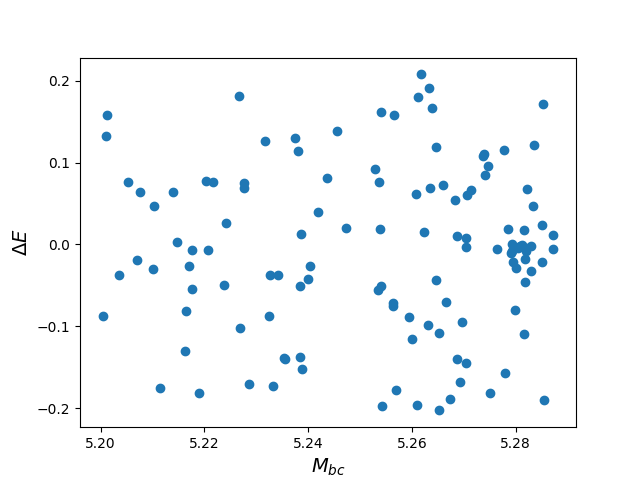
\includegraphics[width=0.7\linewidth]{scatter_2D}
\caption{The 2D scattered plot of $M_{bc}$(GeV) and $\Delta E$(GeV) of data.}
\label{fig:2Dscatter}
\end{figure}
The scattered plots on $M_{bc}$ and $\Delta E$ is shown in Figure \ref{fig:2Dscatter}.
\end{comment}
Using 62.8 fb$^{-1}$ data from the Belle II, we extract the number of signal events to be $N_{sig} = 17.4 \pm 4.2$ from the signal region. The number of background events in the signal region is $7.2\pm 3.6$. The number of signal and background events from the same amount of \textit{generic MC} is calculated to be $\sim$ 20.6 and $\sim$ 4.1.  These values are summarized in Table \ref{tab:recoB}. If we directly count the number of events from the data, there are 30 events in the signal region and 60 events in the sideband region which is defined as $M_{bc} < 5.26 ~ \text{GeV}/c^2$. The events in the signal region will be used as the input data points for the $\it{CP}$ parameters measurement latter. 

 \begin{table}[htpb]
 	\centering 
 	\caption{Reconstructed signal and background events using $M_{bc}$ and $\Delta E$ 2D fit, compared with expected numbers from \textit{generic MC}.}
 	\label{tab:recoB}
 	\begin{tabular}{|c|c|c|} 
 		\hline
 		Events (signal region) & Signal &  Background\\
 		\hline
 		%1 ab$^{-1}$ generic MC fit & $341\pm 20$ & $61 \pm 17$\\
 		%\hline
 		%1 ab$^{-1}$ generic MC expected & $\sim$ 328 & $\sim$ 65\\
 		%\hline
 		%$\sim$ 1 ab$^{-1}$ Belle data &  $327\pm 19$ & $56 \pm 16$\\
 		%\hline
 		62.8 fb$^{-1}$ \textit{generic MC} & $\sim$ 20.6 & $\sim$ 4.1\\
 		\hline
 	    62.8 fb$^{-1}$ data & $17.4\pm 4.2$ & $7.2\pm 3.6$\\
 		\hline
 	\end{tabular}
 \end{table}
 
 
To check reliability of the number of events fitted from the $M_{bc}$ and $\Delta E$ in this low statistics case, we test the 2D fit result, by merging the continuum events and the different number of signal events, to check the linearity of the input and output. From the 2D fit on \textit{generic MC}, the expected number of continuum events in the full range of $M_{bc}$ and $\Delta E$ is $\sim 46$ at 62.8 fb$^{-1}$, which is set to be the constant number of continuum events used in the linearity test. Then the number of signal events from 5 to 30 with 5 events per step are injected into the continuum events, to perform the $M_{bc}$ and $\Delta E$ 2D fit to obtain the output signal events number.
\begin{comment}
For every round of the injection test, the signal and continuum events are randomly sampled into 10 data collection and the 2D fit is performed for each of them. The center value and statistical uncertainty of the fitted number of events are averaged using these 10 results in each injection test.
\end{comment}
The $M_{bc}$ and $\Delta E$ distributions and fit in each injection test are shown in Figure \ref{fig:2Dinject}. The output signal and background events depending on the injected number of the signal events are presented in Figure \ref{fig:2Dinjectline}, where the dependence on both signal and background events are fitted with linear function $y = ax+b$. The error bar on each data point is taken from the statistical uncertainty of the number of signal or continuum events of the 2D fit results. The fit results show a good linearity on the input and output of the number of signal events while the number of continuum events remain close the constant 46 as the input number. The signal events yield from the current luminosity is considered as a reliable result. 


\begin{figure}[htpb]
	\begin{subfigure}{0.5\linewidth}
		\includegraphics[page=1,height=6cm]{figures/injection_sig_5/ds_gen_Mbc_2D.pdf}
		\caption{signal injected: 5}
	\end{subfigure}
	\begin{subfigure}{0.5\linewidth}
		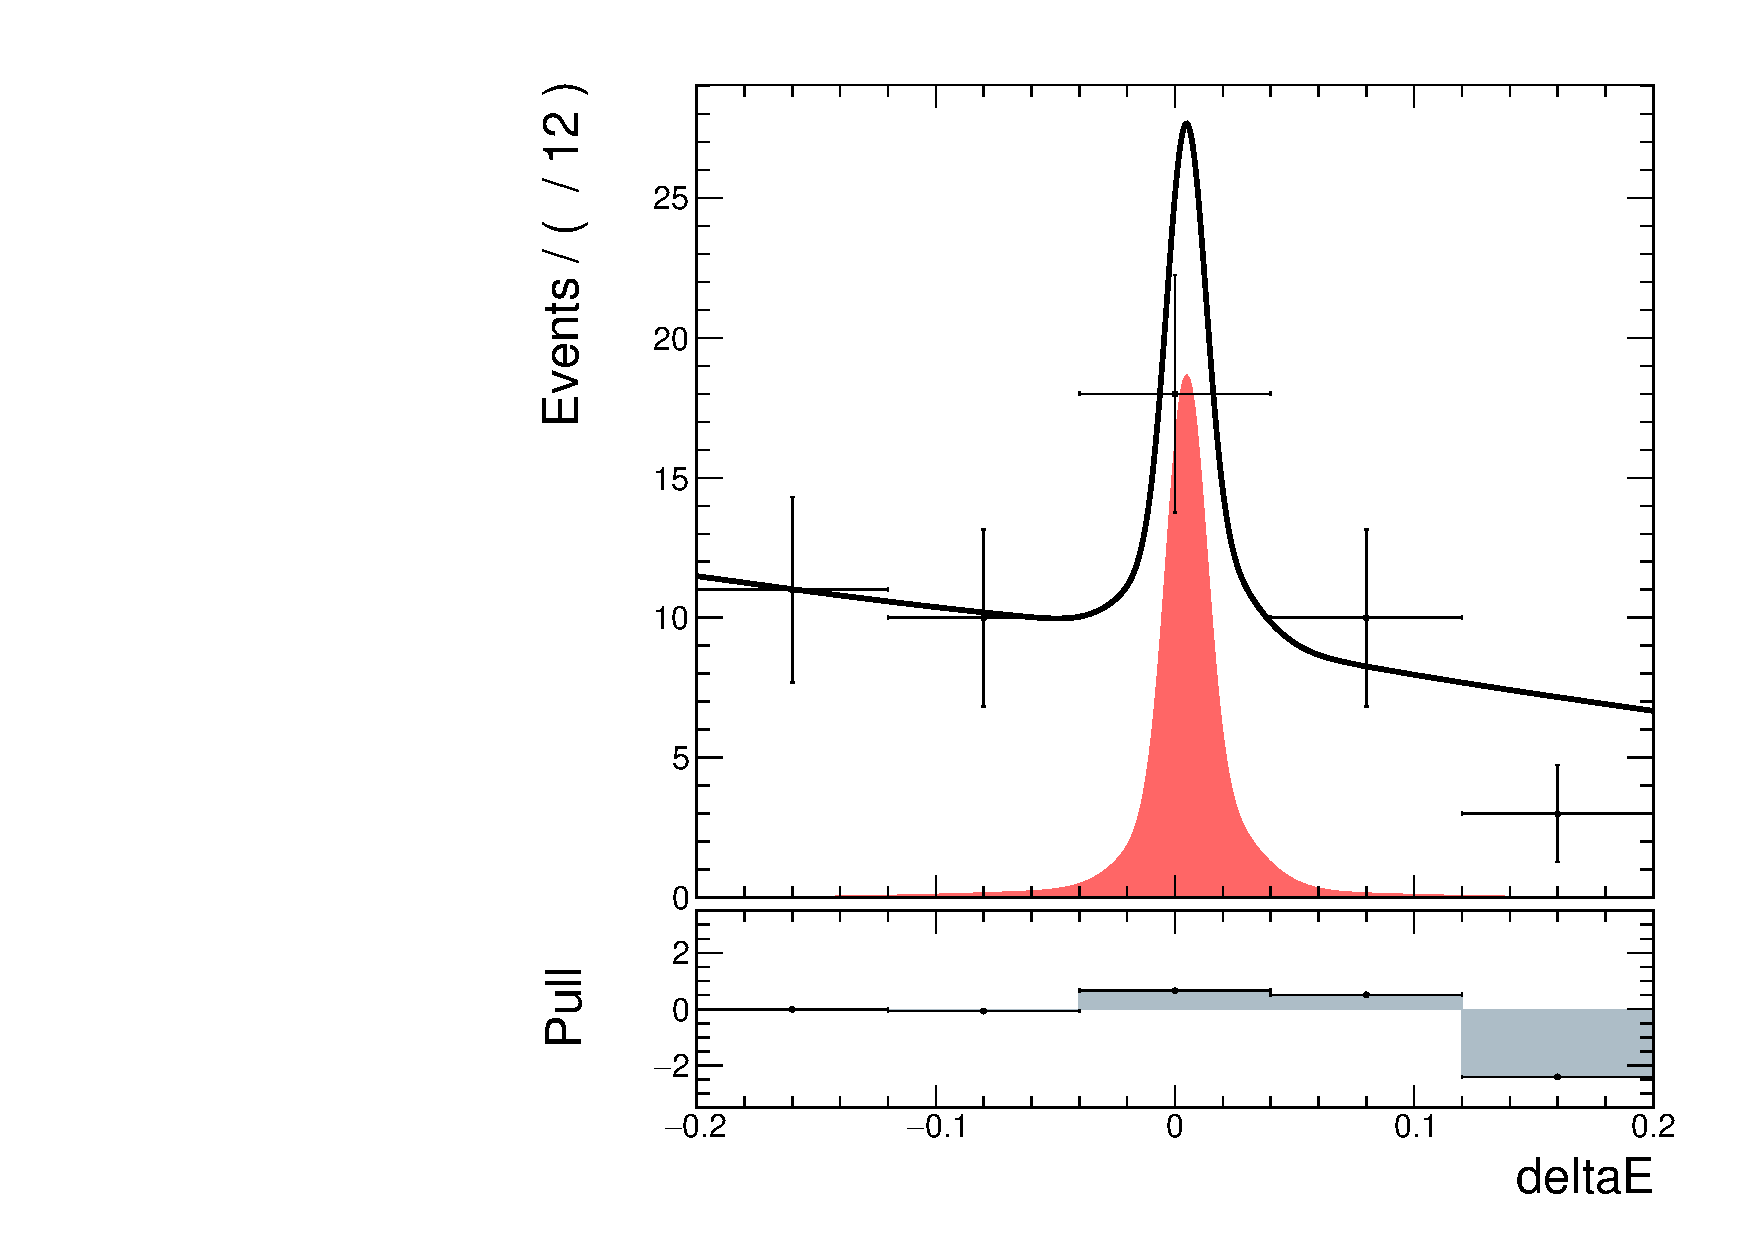
\includegraphics[page=1,height=6cm]{figures/injection_sig_5/ds_gen_deltaE_2D.pdf}
		\caption{signal injected: 5}
	\end{subfigure}
	\begin{subfigure}{0.5\linewidth}
		\includegraphics[page=1,height=6cm]{figures/injection_sig_10/ds_gen_Mbc_2D.pdf}
		\caption{signal injected: 10}
	\end{subfigure}
	\begin{subfigure}{0.5\linewidth}
		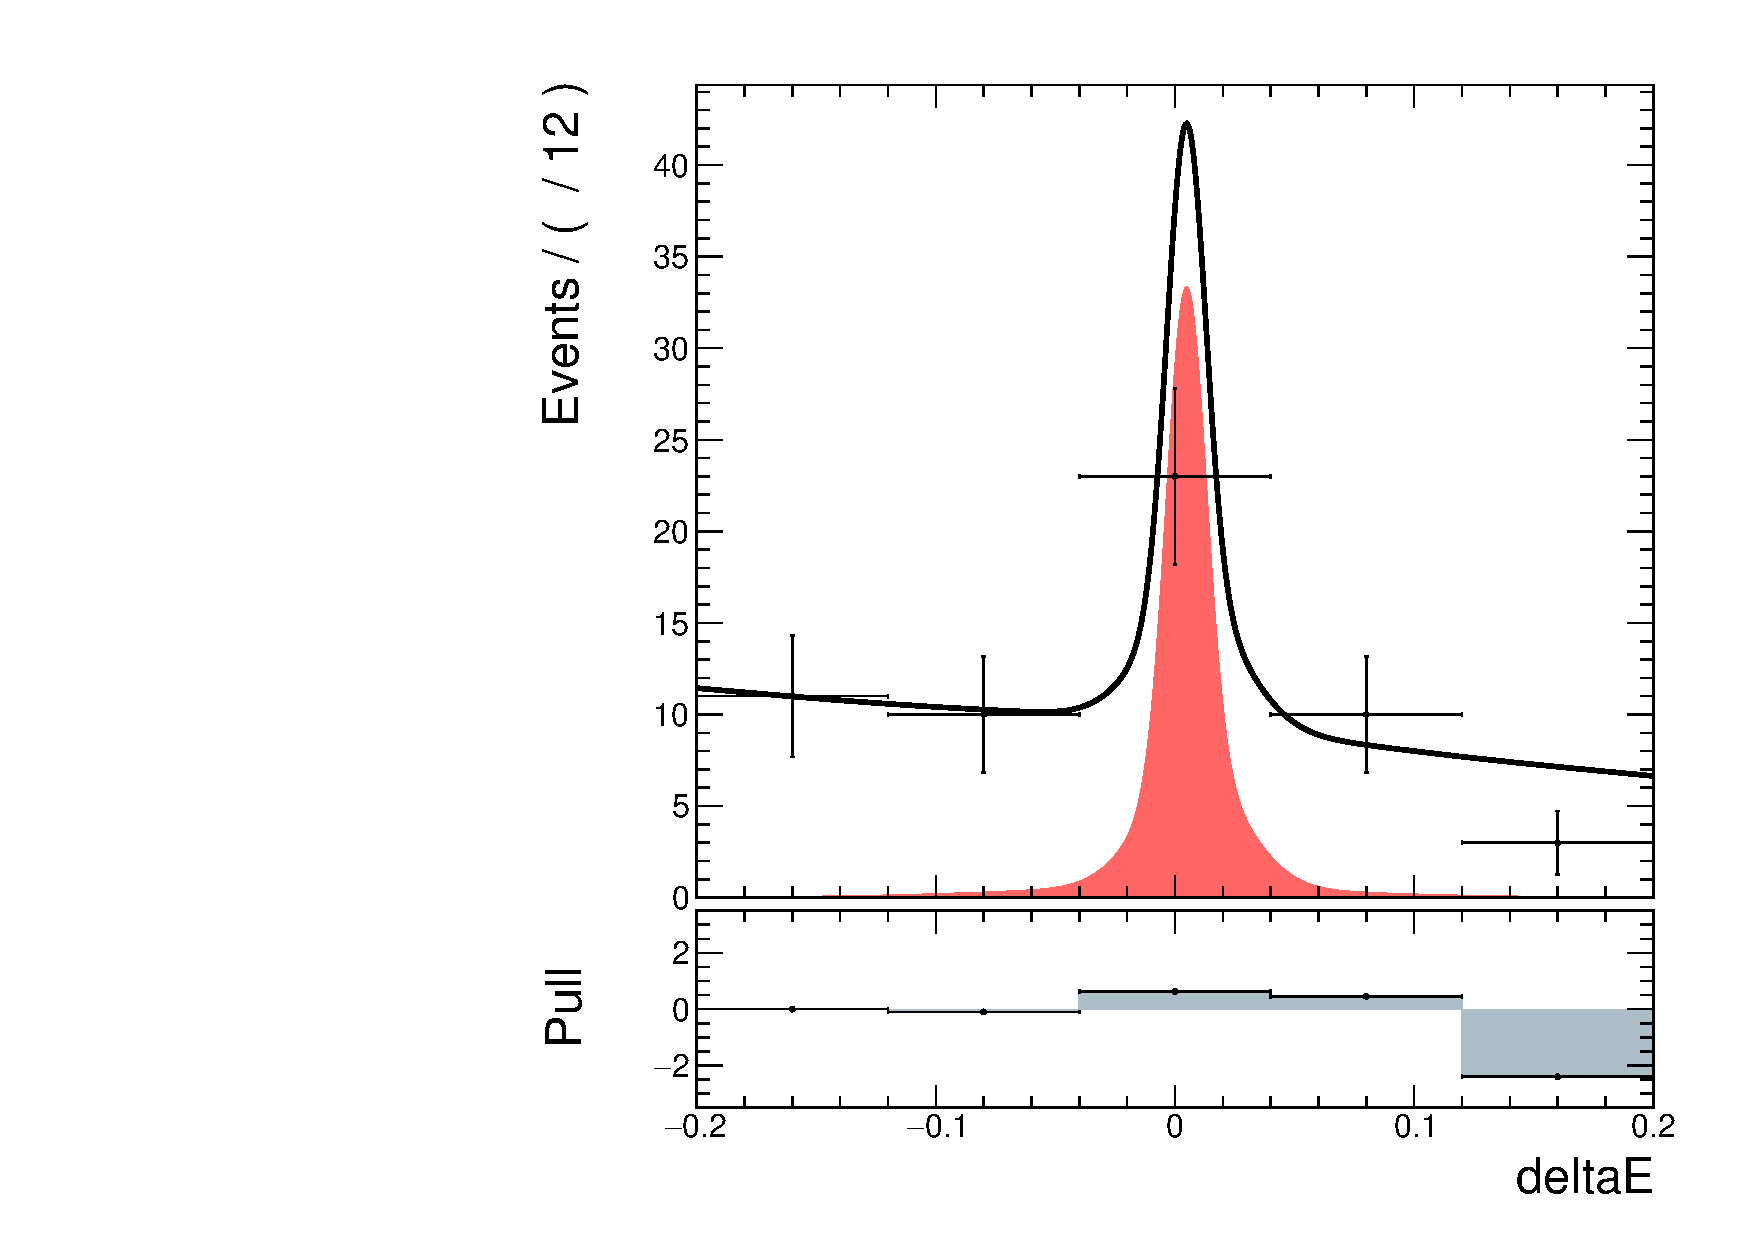
\includegraphics[page=1,height=6cm]{figures/injection_sig_10/ds_gen_deltaE_2D.pdf}
		\caption{signal injected: 10}
	\end{subfigure}
		\begin{subfigure}{0.5\linewidth}
		\includegraphics[page=1,height=6cm]{figures/injection_sig_30/ds_gen_Mbc_2D.pdf}
		\caption{signal injected: 30}
	\end{subfigure}
	\begin{subfigure}{0.5\linewidth}
		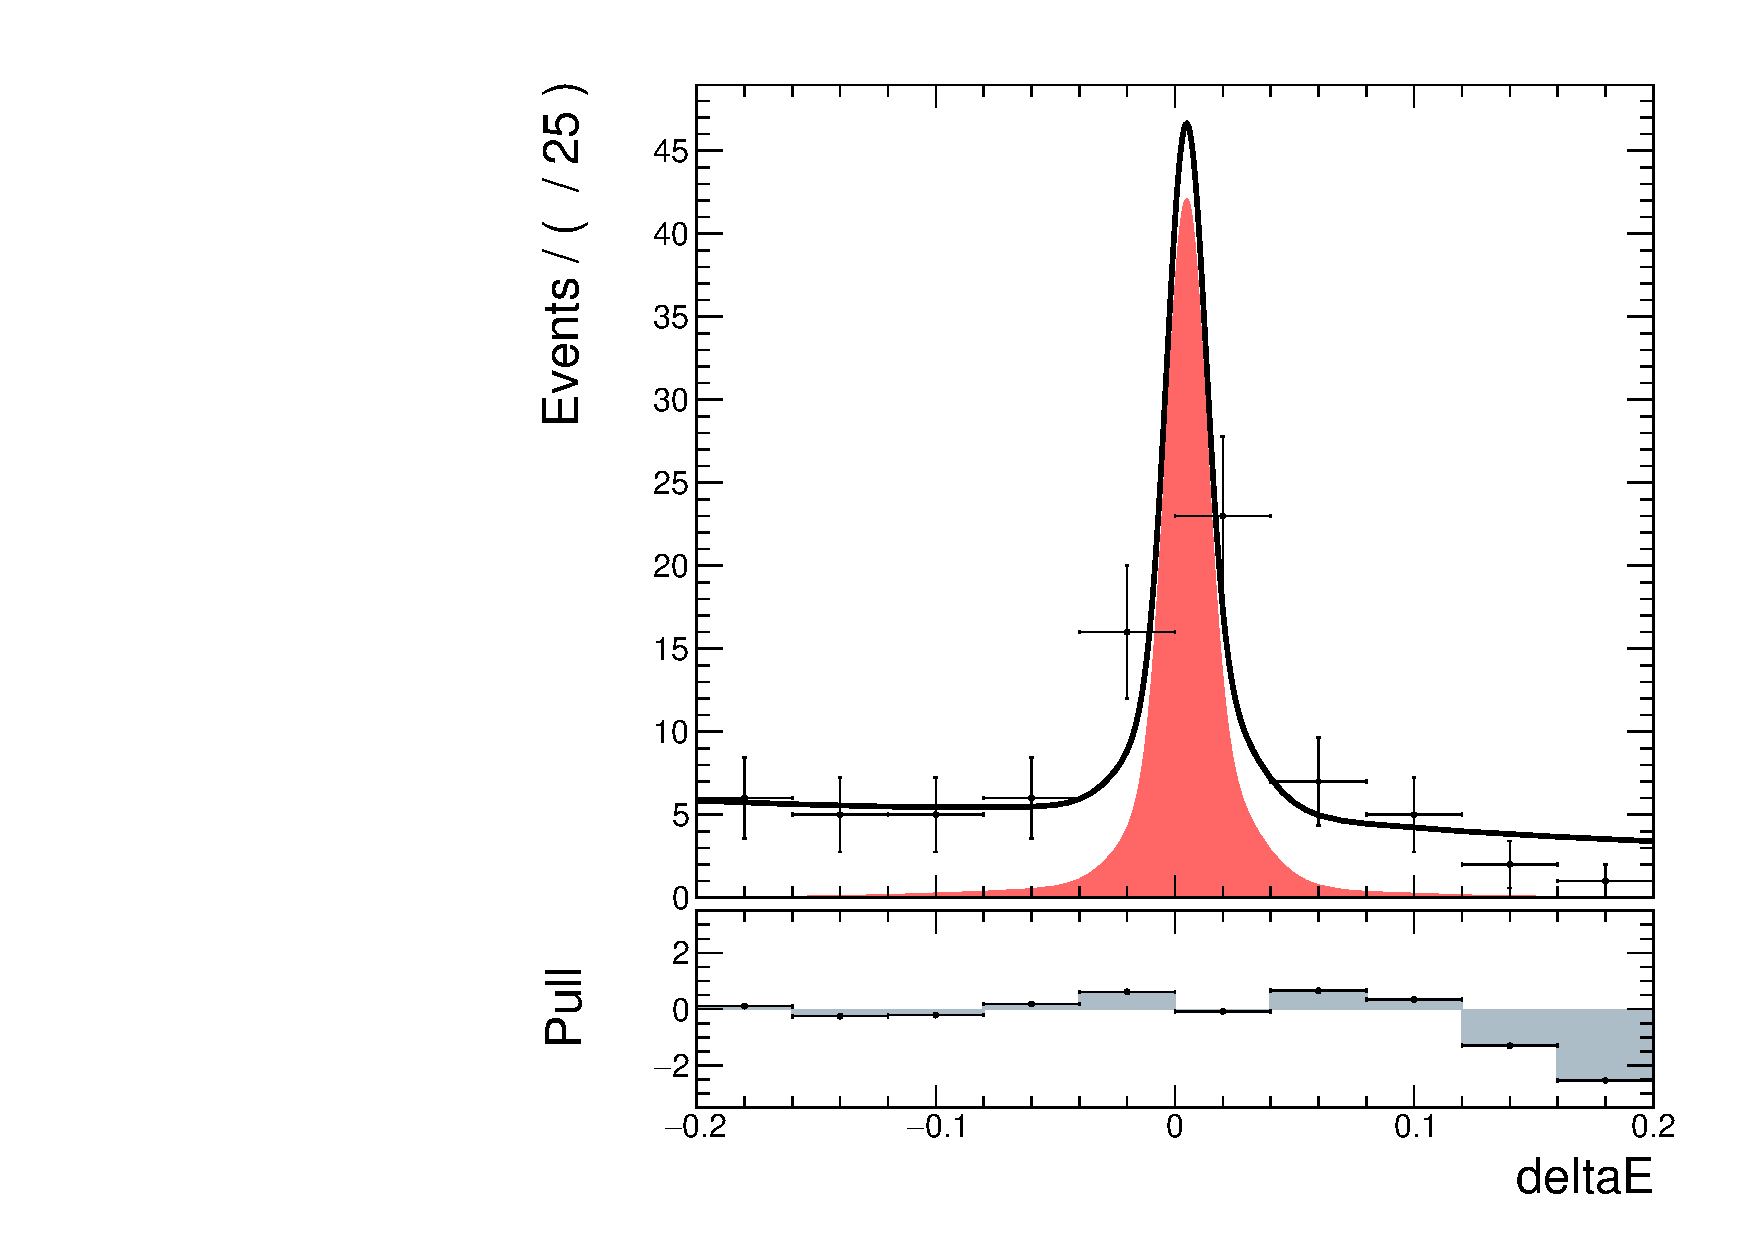
\includegraphics[page=1,height=6cm]{figures/injection_sig_30/ds_gen_deltaE_2D.pdf}
		\caption{signal injected: 30}
	\end{subfigure}
	\caption{The fit results of $M_{bc}$ and $\Delta E$ in signal injection test, where the number of signal events of 5, 10, and 30, injected with 46 continuum events, are shown. The full results including other values of the number of signal events are included in the Appendix D. }
	\label{fig:2Dinject}
\end{figure}


\begin{figure}[htpb]
	\begin{minipage}[b]{0.5\linewidth}
		\centering 
		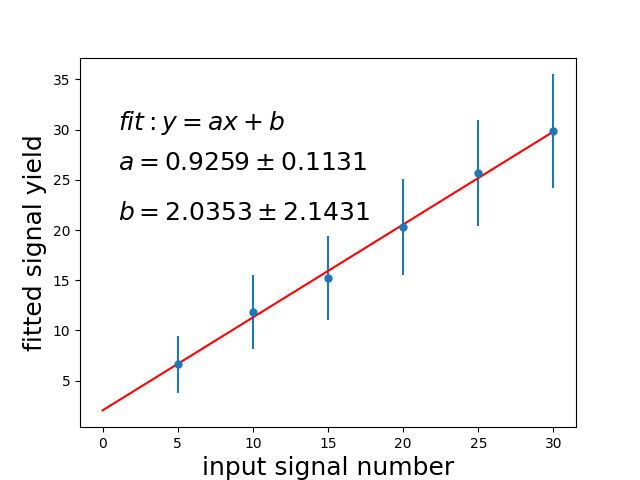
\includegraphics[height=6cm]{figures/inject_line_sig}
		\label{}
	\end{minipage}
	\begin{minipage}[b]{0.5\linewidth}
		\centering 
		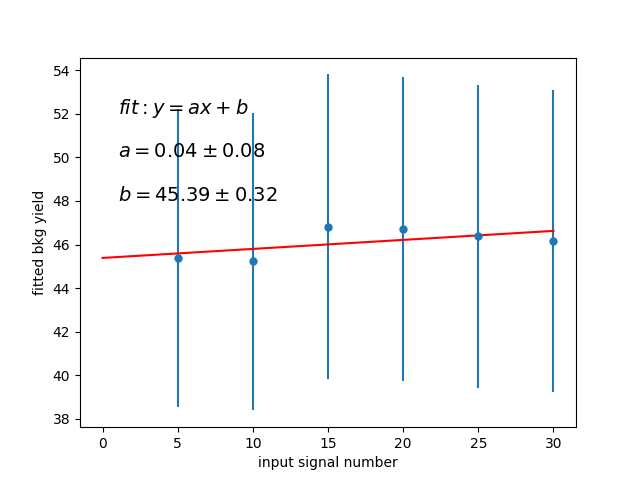
\includegraphics[height=6cm]{figures/inject_line_bkg}
		\label{}
	\end{minipage}
	\caption{Injection test for signal extraction. The linearity is clear between input and output signal events number. The error bar on each point is taken from the statistical uncertainty of the number of signal or continuum events from 2D fit results.}
	\label{fig:2Dinjectline}
\end{figure}

\begin{comment}
\begin{figure}[htpb]
\centering 
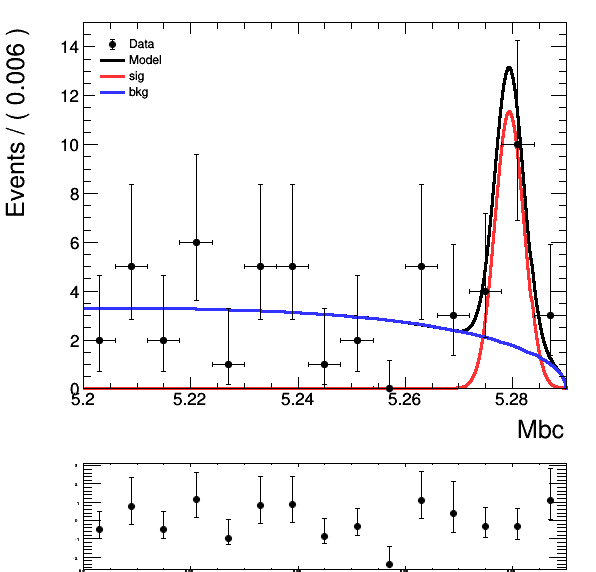
\includegraphics[width=0.7\linewidth]{data-mbc-fit}
\caption{$M_{bc}$ fit in data, signal is Gaussian and background is Argus.}
\end{figure}
\begin{figure}[htpb]
\centering 
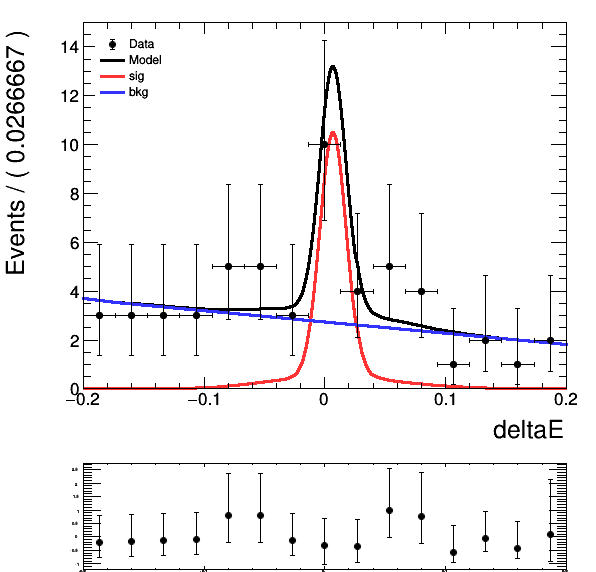
\includegraphics[width=0.7\linewidth]{data-dE-fit}
\caption{$\Delta{E}$ fit in data, signal is double-Gaussian and background is Chebyshev polynomial.}
\end{figure}
\begin{table}[htpb]
\centering
\caption{Fit results from RooFit on $M_{bc}$ and $\Delta E$}
\begin{tabular}{|c|c|c|}
\hline
Floating Parameters  & Mean Value & +/- Error  \\
\hline
N\_sig & 12.8 & 3.93\\
\hline
N\_bkg  & 41.2 & 6.62 \\
\hline
a0 & -0.34 & 0.264\\
\hline
$\chi_{argus}$ & -15.0 & 16.7\\
\hline
\end{tabular}
\end{table}

The fraction of signal and background can be obtained by integral over signal box region using 2D P.D.F. We define signal box using\textit{signal MC} distribution in Fig 4.13 and 4.14, which $5.269 < M_{bc} < 5.287$ GeV and $-0.09 < \Delta E < 0.12$ GeV. The results are: 

\begin{eqnarray}
N_{sigbox} = 12.6 \pm 3.9\\
N_{bkgbox} = 2.6 \pm 0.2 
\end{eqnarray}

Compared with Belle experience, which similar analysis is done by using about 1$ab^{-1}$ data, signal yield is $327.1 \pm 19.4$. The estimated branching fraction of $B^0 \to K_S^0  K_S^0  K_S^0$ is: 
\end{comment}


	


\begin{comment}
\section{Kinematics and Vertexing Dependence on \textit{KsFinder}} 

\textit{KsFinder} largely reduce the combinatorial background of $B^0$ by improving $K_S^0$ purity. 
\begin{figure}[htpb]
\centering
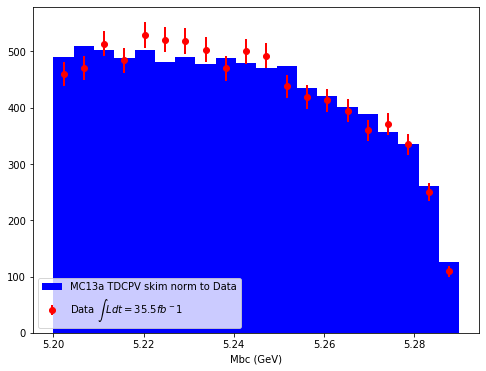
\includegraphics[width=0.7\linewidth]{mbc-noks}
\caption{$M_{bc}$ distribution in data(red) and MC(blue) without $K_S^0$ finder}
\end{figure}
\begin{figure}[htpb]
\centering
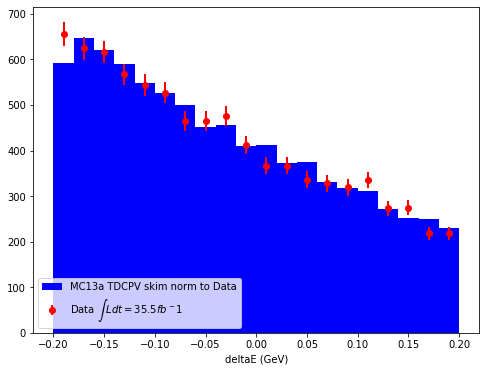
\includegraphics[width=0.7\linewidth]{dE-noks}
\caption{$\Delta{E}$ distribution in data(red) and MC(blue) without $K_S^0$ finder}
\end{figure}


 However, it's essential to check the potential impact on $M_{bc}$ and $\Delta E$, as well as vertex positions on $z$-axis of $B^0$ due the implementation of \textit{KsFinder}. The $K_S^0$ classification uses information such as invariant mass and decay vertex positions which may propagate bias into $B^0$ signal extraction, eventually may affect the measurement of $\it{CP}$ parameters. Given each type of $B^0$ based on how many CDC-only tracks it has in the final states, the comparison on $M_{bc}$ and $\Delta{E}$ with or without \textit{KsFinder} is performed by fitting the distribution in \textit{signal MC}. $M_{bc}$ and $\Delta{E}$ are modeled by signal and double Gaussian, respectively. Comparing corresponding fit results, no clear bias on $M_{bc}$ and $\Delta{E}$ is found by using \textit{KsFinder} where fit results are agreed well within one standard deviation. The fit results are shown in Figure \ref{fig:mbc_bias} and \ref{fig:de_bias}. To be noted, the $\Delta E$ distributions show a small shift positively when more CDC-only tracks are used to reconstructed $B^0$ because the reconstructed energy from charged pions is slightly higher due to the less energy loss in VXD.
 
 \begin{figure}[htpb]
 	\centering
 	\includegraphics[width=0.9\linewidth]{mbc_noKs}
 	\includegraphics[width=0.9\linewidth]{mbc_Ks}
 	\caption{$M_{bc}$ distribution based on the number of CDC-only tracks in final states. Top: no \textit{KsFinder} used; Bottom: \textit{KsFinder} used. The $\mu$ and $\sigma$ are the mean and standard deviation of the Gaussian function.}
 	\label{fig:mbc_bias}
 \end{figure}
 \begin{figure}[htpb]
	\centering
	\includegraphics[width=0.9\linewidth]{dE_noKs}
	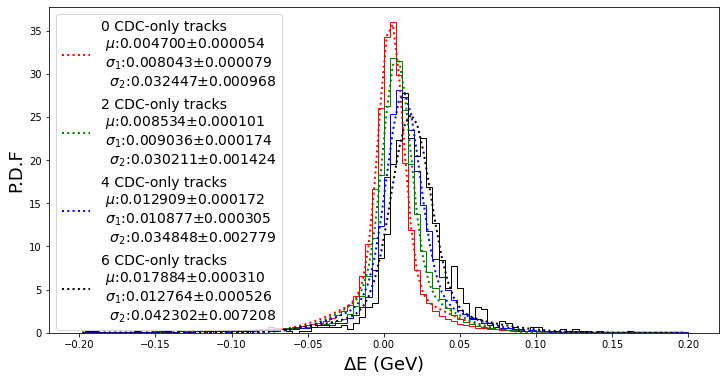
\includegraphics[width=0.9\linewidth]{dE_Ks}
	\caption{$\Delta{E}$ distribution based on the number of CDC-only tracks in final states. Top: no \textit{KsFinder}; Bottom: \textit{KsFinder} used. The $\mu$ is the common mean for double Gaussian. The $\sigma_1$ and $\sigma_2$ are the standard deviations of the Gaussian function.}
	\label{fig:de_bias}
\end{figure}

Similar to the comparison of $M_{bc}$ and $\Delta{E}$, the $z$ direction vertex position and the vertex position difference $\Delta z$ between $\it{CP}$ and tag sides are also checked, in which no clear bias are found either. The $z$ and $\Delta z$ are modeled using single Gaussian with the same mean but different standard deviation. The results are shown in Figure \ref{fig:bias-z} and \ref{fig:bias-zerr}. It is obvious that in Figure \ref{fig:bias-z}, the $\it{CP}$-side resolution of vertex on $z$-axis is wider when the final states of $B^0$ have more CDC-only tracks, especially when all the tracks only contains CDC hits (6 CDC-only tracks).

\begin{figure}[htpb]
	\centering
	\includegraphics[width=0.9\linewidth]{z_noKs}
	\includegraphics[width=0.9\linewidth]{z_Ks}
	\caption{$\Delta z$ distribution based on the number of CDC-only tracks in final states. Top: no \textit{KsFinder}; Bottom: \textit{KsFinder} used. The $\mu$ and $\sigma$ are the mean and standard deviation of the Gaussian function.}
	\label{fig:bias-z}
\end{figure}
\begin{figure}[htpb]
	\centering
	\includegraphics[width=0.9\linewidth]{dz_noKs}
	\includegraphics[width=0.9\linewidth]{dz_Ks}
	\caption{$\Delta z$ distribution based on th number of CDC-only tracks in final states. Top: no \textit{KsFinder}; Bottom: \textit{KsFinder} used. The $\mu$ and $\sigma$ are the mean and standard deviation of each Gaussian function.}
	\label{fig:bias-zerr}
\end{figure}
Above all, no clear appearance of bias on $M_{bc}$ and $\Delta E$ distributions, as well as vertex positions from using \textit{KsFinder} has been found, \textit{KsFinder} may implement a small shift on the vertex position which is negligible compared to the large statistical uncertainty due to the current low luminosity. Hence, there's no correction on these observables are applied in this analysis, and the systematic uncertainty from \textit{KsFinder} is evaluated by taking into account of $R_{B^0}$ in signal fraction calculation.
\end{comment}